\documentclass[11pt, a4paper, twoside]{book}

\setlength{\topmargin}{2pt} \setlength{\headheight}{15pt}
\setlength{\headsep}{25pt} \setlength{\textheight}{640pt}
\setlength{\footskip}{25pt}
\setlength{\hoffset}{0pt}
\setlength{\oddsidemargin}{0pt} \setlength{\oddsidemargin}{3pt}
\setlength{\evensidemargin}{0pt} \setlength{\evensidemargin}{30pt}
\setlength{\textwidth}{430pt}
\setlength{\marginparsep}{0pt} \setlength{\marginparwidth}{0pt}
\usepackage[french]{babel}
\usepackage[utf8]{inputenc}
\usepackage[T1]{fontenc}
\usepackage[autolanguage]{numprint}
\usepackage{hyphenat}
\hyphenation{mathéma-tiques récu-pérer}
\usepackage{graphicx}
\graphicspath{ {images/} }
\usepackage[margin=1.25in]{geometry}
\usepackage{longtable}
\usepackage{float}
\usepackage{textcomp}
\usepackage{amsmath}
\usepackage{pdfpages}
\usepackage{nomencl}
\usepackage{lettrine}
%start of title
{\title{
%include the logo
ÉCOLE NATIONALE DES SCIENCES APPLIQUÉES DE KÉNITRA \\  \vspace*{1truecm} Moroccan foundation for Advanced Science, Innovation and Research \\ 
(MAScIR) \\
\vspace*{1truecm} Rapport de Projet de Fin d'Étude \\ \vspace*{0.5truecm} \textbf{Étude et réalisation d'un système RFID}} 
%end of title

\author{Réalisé par : \\ Otmane BOUAYAD \vspace*{1truecm} \\ Encadré par : \\
Mme Ilham BOUZIDA : Encadrante professionnelle\\ 
Pr Tomader MAZRI : Encadrante académique\\
}
\date{(Du 15 Février au 30 Juin  2016)}

\begin{document}

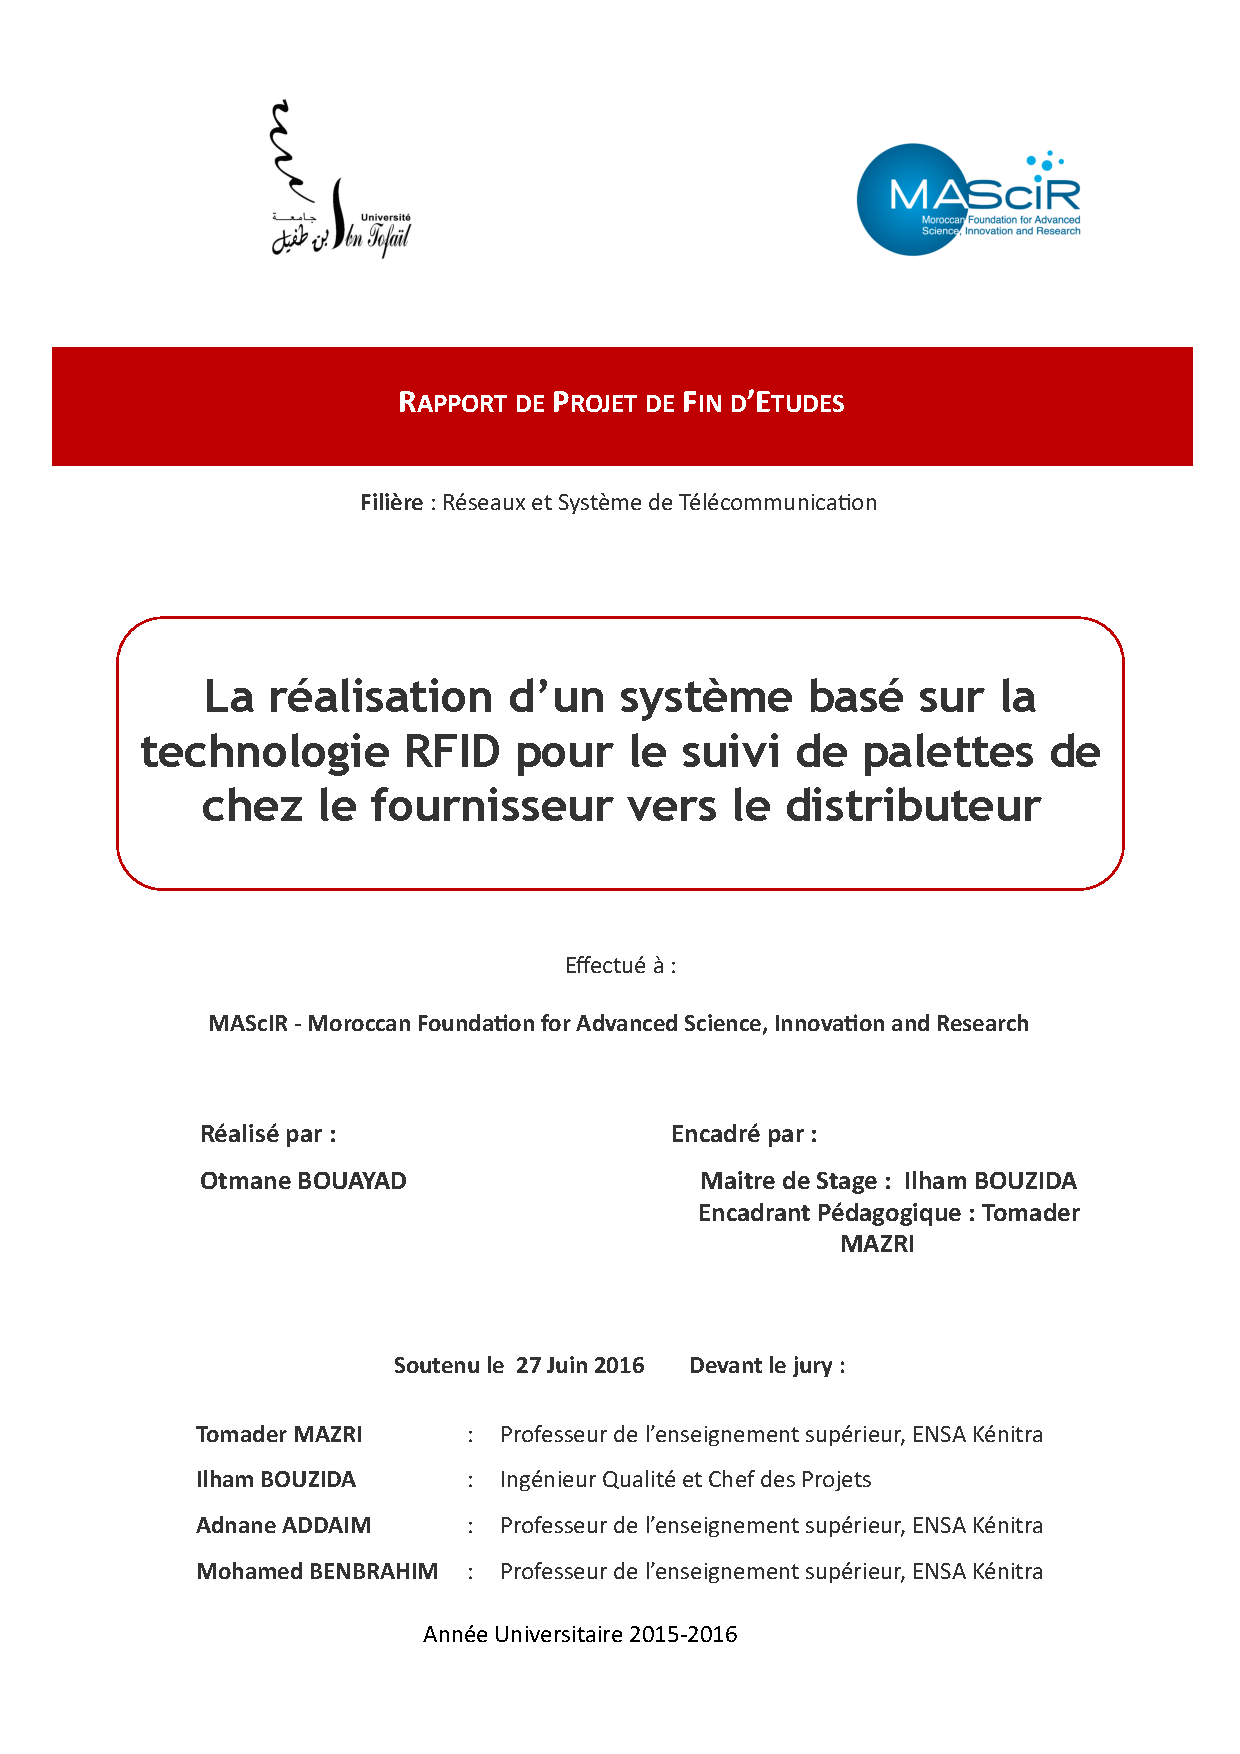
\includepdf[pages=1]{pagedegarde2016.pdf}
\maketitle
\pagestyle{plain}
%Dedicas
\frenchspacing
\chapter*{Dédicace}

I would like to dedicate this work to my wife, Oumaïma, for her love, encouragement, and continuous support,my parents, who has thought me many things in life, including the one motto I live by: 
\emph{“Never give up on your dreams. Hard work and diligence will see you through as long as you never give up.”}
 So it is with all my love, respect, and admiration that I dedicate this to you.My sister and my best friends forever Reda and Nouhaila,my future engineers. Remember
\emph{“Accomplishment is product of thoughts, mind is everything”.}

%remerciment
\chapter*{Remerciements}
\addcontentsline{toc}{section}{Remerciements}
\emph{
Avant tout développement sur cette expérience professionnelle, il apparaît opportun de commencer ce rapport de stage par des remerciements, à ceux qui m'ont beaucoup aidé au cours de ce stage, et à ceux qui ont eu la gentillesse de faire de ce stage un moment très profitable.\\}

\emph{
Aussi, je tiens plus particulièrement à remercier Mme Ilham
BOUZIDA, ingénieur qualité dans l’équipe packaging à MAScIR, et M. Brahim LAKSSIR, directeur de service packaging à MAScIR, mes encadrants industriels qui m'ont accompagné patiemment tout au long de ce stage. Je remercie l'ensemble des employés de la Fondation MAScIR pour les conseils qu’ils m'ont prodigué au cours de ce stage.\\}

\emph{Je souhaite remercier mon promoteur et mon encadrant à l'école Pr. Tomader MAZRI pour ses instructions et son aide lors du stage.\\}

\emph{Finalement ,Je remercie Pr. Adnane ADDAIM, Pr. Tomader MAZRI et Pr. Mohamed BENBRAHIM de m’avoir fait l’honneur d’accepter d’évaluer ma mémoire. Je suis également honoré de votre participation à mon jury de soutenance, malgré votre emploi du temps surchargé. Je vous remercie aussi pour votre regard critique. Cela va m'apporter sans doute des éclairages intéressants, et me permettra de soulever certaines interrogations pour poursuivre ma réflexion dans des travaux de recherche futurs. \\ }

\emph{Enfin, j’adresse tous mes remerciements les plus sincères à tous les enseignants de l’ENSA de Kénitra pour avoir contribué à la formation que j’ai acquise lors de mon cursus.}
%include the table of content please
\tableofcontents

%include the liste of figure please
\listoffigures

\listoftables

\chapter*{Introduction}
\addcontentsline{toc}{section}{Introduction}
Le terme RFID \footnote{Radio Frequency Identification} englobe toutes les techniques qui utilisent les ondes radio pour identifier automatiquement les objets ou les personnes. Le système RFID autrement dit l'identification par radio fréquence est une technique qui permet de mémoriser et de récupérer les informations à distance grâce à une étiquette qui émet des ondes radio.\\

Le système RFID (audiofréquence identification) est une technique très attractive pour l'entreprise qui offre la possibilité d'une gestion automatique du nombre conséquent d'informations qu'elle doit traiter. Les équipements adaptés à ce système permettent de synchroniser les flux physiques avec les flux d'informations.\\

Dans le cadre du projet de fin d'études, j'ai eu l'opportunité de travailler sur cette technique avec la fondation MAScIR qui occupe une position leader sur le marché de la recherche en micro-électronique.\\

Ce projet porte alors, sur l'étude et la réalisation d’une solution RFID UHF \footnote{Ultra High Frequency} qui assure l’identification et la traçabilité des entrées et sorties des palettes. Choisir les tags adaptés aux besoins en respectant les conditions d’utilisation et le type du lecteur. Développer un logiciel de gestion des palettes. D’autre part, la réalisation d’un transpondeur RFID UHF et une application Android pour la gestion du secteur d'agriculture.\\

Le rapport que je présenterai est organisé en 4 chapitres.


\begin{itemize}
\item Chapitre 1: En premier lieu je vais commencer par une présentation de l'entreprise d'accueil, les services crées pour répondre au besoin de l'industrie marocaine. Ensuite je vais introduire la structure hiérarchique et le département microélectronique où mon stage a eu lieu, notre mission, nos laboratoires et nos équipements. Finalement une description du contexte général du projet et du déroulement du stage.

\item Chapitre 2: Généralité sur la technologie RFID, dans ce chapitre je vais  présenter les composants d'un système RFID, la différence dans la bande de fréquences de rayonnement et son impact sur leur domaine d'utilisation. je vais ensuite présenter les différent type de tag et leur fonctionnalité

\item Chapitre 3: Les solutions proposées et étude théorique, dans ce chapitre je vais présenter les solutions que j'ai ramené pour répondre au besoin de l'entreprise. En premier lieu, le middlware et l'application desktop qui permettent de stocker les informations lues par le lecteur dans une base de données puis les présenter à l'utilisateur d'une maniéré claire. En deuxième lieu la solution RFID Android qui permet la gestion et le suivi des vaccins pour les animaux de production. Finalement un transpondeur RFID miniaturisé pour les tags d'identification.

\item Chapitre 4: Réalisation et simulation, dans ce chapitre je vais présenter tous les résultats et simulation des différentes solutions avec une description détaillée de toutes les fonctionnalités et les possibilités que les produits permettent à l'utilisateur.
\end{itemize}

\pagestyle{plain}

\chapter{Entreprise d'accueil et déroulement du stage}
\pagestyle{headings}
\section{Présentation générale de MAScIR}
MAScIR\footnote{Moroccan foundation for Advanced Science, Innovation and Research} est un organisme de recherche à caractère scientifique et technologique. Il est voué à la recherche en nanotechnologie, en biotechnologie, en technologie numérique, en micro-électronique, en énergie et en environnement. La fondation se veut présenter là où les enjeux de la société l’exigent.\\

La figure suivante montre emplacement de l’entreprise.

\begin{figure}[h]
\centering
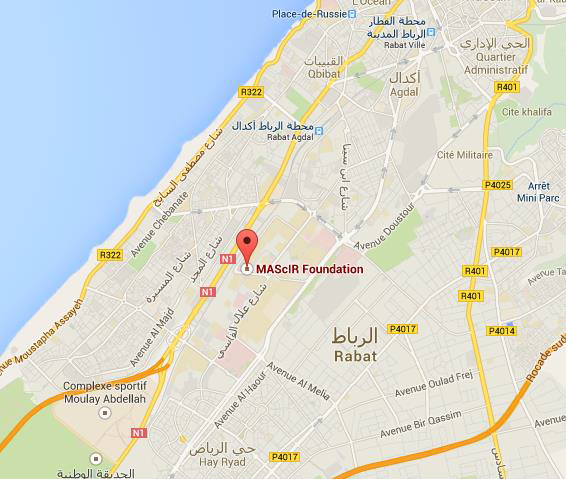
\includegraphics[width=0.75\textwidth]{mascir_map}
\caption{Localisation de la fondation MAScIR}
\end{figure}

Rassemblant d’éminents chercheurs des quatre coins du monde, MAScIR regroupe des équipes scientifiques œuvrant dans des domaines innovants et complémentaires et met à leur disposition une infrastructure scientifique de pointe.\\

Initialement fondée en 2007 par le gouvernement marocain en tant que fondation à but non lucratif MAScIR a continuée son expansion en créant :

\begin{description}
\item[MAScIR MicroElectronics] a pour objectif de devenir un centre de recherche et développement dans le domaine de la microélectronique.
\item[MAScIR BioTechnology] deuxième centre inscrit dans MAScIR œuvrant dans le domaine de la biotechnologie : recherche et développement des médicaments ou des biocides.
\item[NanoTechnology] qui a pour mission de mener des recherches appliquées, innovantes et à la fine pointe de la technologie dans le domaine des nanomatériaux et des nanotechnologies. Ces recherches sont menées par une équipe internationale du haut calibre travaillant dans un environnement unique et utilisant une infrastructure de pointe.
\end{description}

\subsection{Client de la fondation}
Les principaux clients de la fondation MAScIR MicroElectronics sont :
\begin{description}
\item[Lear Corporation] est l’un des principaux fournisseurs mondiaux de sièges automobiles et des systèmes de gestion de l’énergie électrique.
\item[ONCF] est l'opérateur ferroviaire national du Maroc. Le Bureau emploie environ 7845 employés et possède un réseau de 2110 km, tous les 1435 mm (4 pi 8 1/2 po) à écartement standard, dont 1300 km est électrifié (2015).
\item[OCP] est un acteur incontournable sur le marché du phosphate et de ses produits dérivés. Présent sur toute la chaîne de valeur, il est le premier exportateur de cette matière dans le monde.
\item[COSUMAR] est un groupe marocain, filiale de la société nationale d'investissement, spécialisé dans l'extraction, le raffinage et le conditionnement du sucre sous ses différents formes. Il est devenu l'unique opérateur sucrier marocain après l'acquisition de SUTA, SUCRAFOR, SUNABEL et SURAC en 2005.
\item[STERIMED] est une société spécialisée dans le domaine de l’eau et des technologies de l’environnement. Son objectif est d’accompagner les entreprises et participer dans la résolution des problématiques liées à l’eau et l’environnement.
\end{description}

\subsection{Structure et hiérarchie}
La fondation est gérée par un conseil d’administration qui  investi dans la gestion. Le conseil dispose de quatre comités distincts : un comité d’investissement, un comité de suivi, un comité de vérification et un comité de Rémunération; qui assurent une gestion rapprochée des sujets relatifs à leur mission.
\begin{description}
\item[Conseil d'administration] détermine les orientations stratégiques de MAScIR et veille à leur mise en œuvre dans des réunions réguliers. En prenant des décisions, le conseil compte sur le travail des comités spécialisés.
\item[Comité de vérification] le rôle principal du comité d'audit est de permettre à la commission de veiller sur la qualité des contrôles internes et l'intégrité de l'information divulguée aux intervenants et aux partenaires.
\item[Comité des rémunérations] est responsable de faire des recommandations au conseil sur la nomination des administrateurs. Il est également responsable de l'examen de la politique en matière de rémunération de la haute direction au sein de MAScIR.
\item[Comité de suivi] surveille la mise en œuvre effective et correcte des projets dans le cadre de l'accord signé entre MAScIR et le gouvernement marocain.
\item[Comité d'Investissement] assiste le conseil d'administration dans l'accomplissement de sa responsabilité de surveillance pour les actifs d'investissement liés à l'équipement scientifique.
\end{description}

\section{Présentation du département microélectronique}
MAScIR Micro est un centre d’innovation et de développement de la technologie dans le domaine de la microélectronique. Il se focalise sur la simulation, les tests, le design, le packaging, la qualification et le prototypage des produits microélectroniques.
\subsection{Mission}
Le programme Microélectronique a réuni une équipe de direction de classe mondiale pour assurer la traction initiale sous licence des technologies de pointe qui sont disponibles pour une utilisation immédiate. \\

MAScIR Micro fournit des services pour des clients industriels, mais elle développe aussi son propre business dans les domaines suivants :
\begin{itemize}
\item L’intégration et la miniaturisation des systèmes microélectroniques.
\item L’analyse de fiabilité et défaillance des produits.
\item Modélisation des systèmes complexes.
\item Prototypage et industrialisation des produits innovants.
\item Industrialisation des idées et résultats académiques.
\end{itemize}

\subsection{Laboratoires}
Le département microélectronique de MAScIR possède plusieurs laboratoires équipés de technologie avancée :
\begin{itemize}
\item Salle blanche
\item Laboratoire de fiabilité et analyse de défauts
\item Laboratoire électronique\\\\\\\\\\\\\\\\\\\\
\end{itemize}

\begin{figure}[H]
\centering
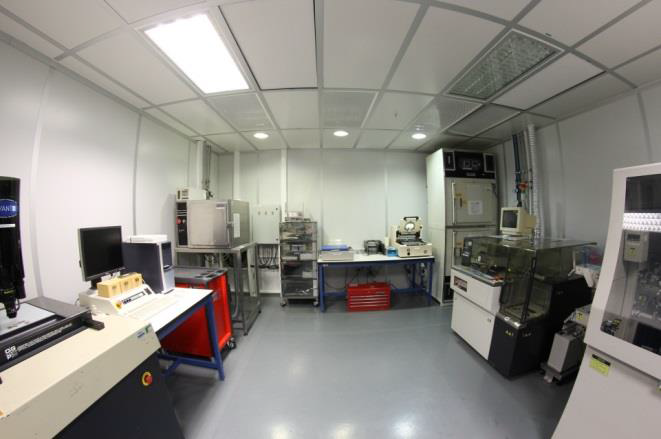
\includegraphics[width=0.75\textwidth]{cleanroom}
\caption{Salle blanche}
\end{figure}

\begin{figure}[H]
\centering
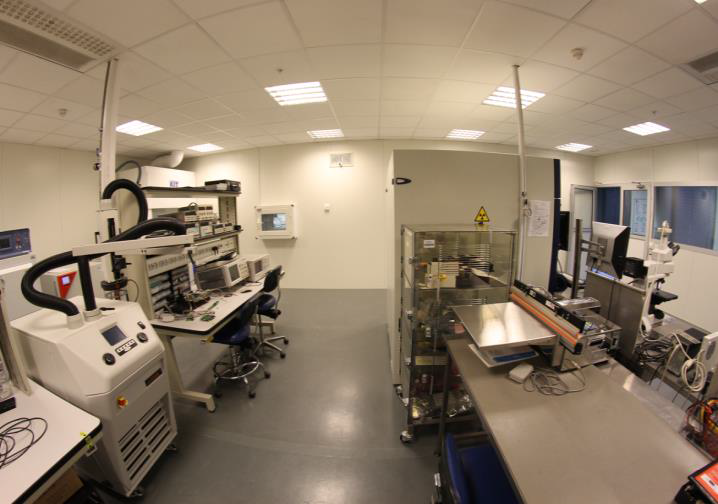
\includegraphics[width=0.75\textwidth]{labo}
\caption{Laboratoire de fiabilité et analyse de défauts}
\end{figure}

\subsection{Équipements}
\begin{itemize}
\item Ligne CSP \footnote{Chip Scaled Packaging}
\item Ligne SMT \footnote{Surface Mount Technology}
\item SAM \footnote{Scanning Accoustic Microscope}
\item X-Ray
\item Chambres climatiques
\end{itemize}

Pour plus d'informations, visiter le site de l'entreprise : \texttt{http://www.mascir.ma}.


\section{Contexte Général du projet}
Le but de cette section est de présenter la problématique du projet, le cahier des charges, la démarche suivie pour répondre au besoin de l’ensemble des parties prenantes du projet et le plan d’action.

\subsection{Objectif}
L’objectif de ce projet est l'étude et la réalisation d’une solution RFID UHF qui assure l’identification et la traçabilité des entrées et sorties des palettes. Choisir les tags et type de lecteur adaptés aux besoins en respectant les conditions d’utilisation et  développer un logiciel de gestion des palettes. 
Et comme deuxième axe, la réalisation d’un transpondeur RFID UHF et une application Android pour la gestion du secteur d'agriculture qui permet à l’utilisateur de profiter des fonctions offertes par les systèmes à distance. \\
\subsection{Cahier des charges}
Assurer l’identification et la traçabilité des entrées et sorties des palettes
\begin{itemize}
\item Choix des tags adaptés aux besoins, conditions d’utilisation et type de lecteur.
\item Établir un programme de gestion des palettes en assurant la traçabilité de leur mouvement.
\item Réalisation et test d’un prototype.\\
\end{itemize}
\subsection{Mise au point de la problématique}
Ce projet consiste à développer un système de traçabilité des entrées et sorties des palettes. Trouver les causes racines et choisir des solutions optimales pour un problème ou une situation nécessitent une grande compréhension du problème. Dans ce sens, la méthode QQOQCP \footnote{Qui ? Quoi ? Où ? Quand ? Comment ?  Pourquoi ?} et le diagramme pieuvre permettent d'avoir des informations élémentaires suffisantes sur toutes les dimensions du problème, pour identifier ses aspects essentiels.\\\\\\\
        
\begin{longtable}{|l|c|}
  \hline
  Quoi & Activité : Développement d’un un système de traçabilité \\
       &  Produit : logiciel , Application Android, Tag UHF \\
  \hline
  Qui & Client MAcIR\\
  \hline
  Où & MAcIR\\
  \hline
  Quand & Du 15/02/2016 au 30/06/2016\\
  \hline
  Comment & État d’art sur les techniques RFID \\
          &  existantes afin de développer une autre plus adaptée.\\
  \hline
  Pourquoi & Fournir un système de traçabilité des entrées et sorties des palettes.\\
  \hline
  
\caption{Étude du besoin}
\end{longtable}

\begin{figure}[H]
\centering
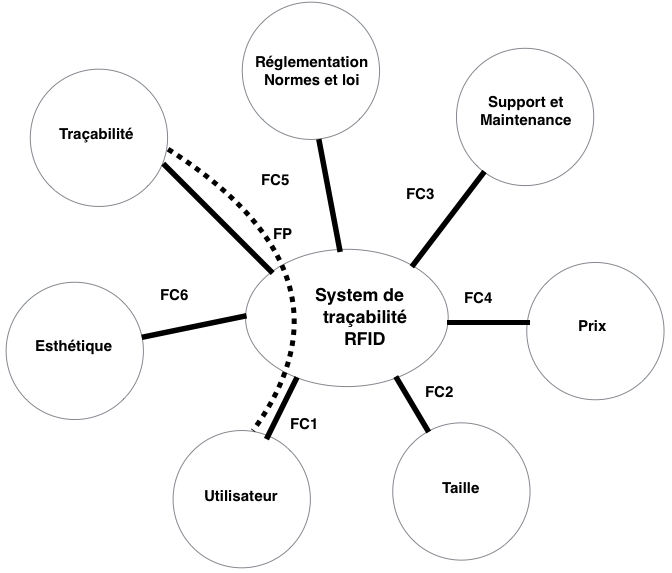
\includegraphics[width=9cm,height=8cm]{pieuvre}
\caption{Diagramme pieuvre}
\end{figure}


\begin{longtable}{|c|c|}
\hline
\textbf{Fonction} & \textbf{Description} \\
\hline
FP & Assurer la traçabilité des palettes de l'entrée vers la sortie  \\
\hline
FC2 & Concevoir un produit de petite taille  \\
\hline
FC3 & Élaborer un plan de support et de maintenance  \\
\hline
FC4 & Réduire le coût   \\
\hline
FC5 & Respecter la réglementation et la loi marocaine \\
\hline
FC6 & Simple et claire à utiliser \\
\hline
FC7 & Assurer le stockage des données et faciliter l'accès aux informations \\
\hline
\caption{Table des fonctions}
\end{longtable}



\subsection{Décomposition du projet}
Le projet se compose principalement de 3 parties :
\begin{itemize}
\item Développement du Middleware et de l'interface graphique: une partie qui consiste à assurer la communication entre le client et le lecteur RFID ,puis visualiser les données lues à l'utilisateur.
\item Développement de l'application SmartFlah pour la gestion des tags animal.
\item Le transpondeur : la conception d'un transpondeur UHF RFID de petite taille.\\
\end{itemize}
Chaque partie sera étudiée indépendamment dans les chapitres qui suivent.
\section{Activités et déroulement chronologique du stage}
\subsection{Activités exercées}
Durant ce stage de fin d’études, j’ai eu l’opportunité de côtoyer le monde industriel et plus précisément de la microélectronique ce qui m’a permis d’assister et participer à plusieurs missions et projets que ça soit au sein de MAScIR ou à l’extérieur. Mis à part le travail sur mon projet, j’ai pu suivre le processus du packaging allant du découpage wafer au marquage boîtier et sciage. Parallèlement, j’ai assisté à des manœuvres de vérification de qualité des produits livrés à MAScIR. Par ailleurs, j’ai pu bénéficier d’un encadrement étroit en préparant des réunions pour garantir un bon état d’avancement du projet.

\subsection{Répartitions des tâches}
%you need to revise mistakes
\noindent
\textsc{1\textsuperscript{ère} et 2\textsuperscript{ème} semaine :}
\begin{itemize}
\item Visite du local et réunions pour cerner le projet.
\item Bibliographie sur les systèmes RFID.
\end{itemize}
\textsc{3\textsuperscript{ème} et 4\textsuperscript{ème} semaine :}
\begin{itemize}
\item Étude du marché et choix des tags et lecteurs RFID.
\item Participer à la résolution des problèmes du lecteur existant.
\end{itemize}
\textsc{5\textsuperscript{ème} et 6\textsuperscript{ème} semaine :}
\begin{itemize}
\item Étude et familiarisation avec le langage \emph{.NET  C\#}
\item Réalisation d'un prototype de test de lecture des tags.
\end{itemize}
\textsc{7\textsuperscript{ème} et 8\textsuperscript{ème} semaine :}
\begin{itemize}
\item Proposition d'un algorithme d'amélioration des performances de la communication client-lecteur
\item Implémentation finale du prototype du nouveau protocole de communication client lecteur.
\end{itemize}
\textsc{9\textsuperscript{ème} semaine :}  
\begin{itemize}
\item Développement d'une interface utilisateur pour le contrôle du flux des données et gestion du stockage.
\item L'étude du marché marocain de l'agriculture et l'étude des besoins .
\end{itemize}
\textsc{10\textsuperscript{ème} et 11\textsuperscript{ème} semaine :}
\begin{itemize}
\item Développement de la version une de l'application SmartFlah.
\item Amélioration de la version une de l'application SmartFlah
\end{itemize}
\textsc{12\textsuperscript{ème} et 13\textsuperscript{ème} semaine :}
\begin{itemize}
\item Étude profonde des tags RFID UHF.
\item Réalisation du 1er prototype d'antenne UHF RFID
\end{itemize}
\textsc{14\textsuperscript{ème} et 15\textsuperscript{ème} semaine :}
\begin{itemize}
\item Étude des méthodes d'optimisation de la taille et des performances des antennes.
\item simulation sur CST studio du 2ème prototype d'antenne
\end{itemize}
\textsc{16\textsuperscript{ème} et 17\textsuperscript{ème} semaine :}
\begin{itemize}
\item simulation sur CST studio du 3ème prototype d'antenne
\item Rédaction du rapport\\\\\\\\\\\\\
\end{itemize}
\pagebreak
\subsection{Étapes	de réalisation}
\begin{longtable}{|p{0.35\textwidth}|p{0.2\textwidth}|p{0.2\textwidth}| p{0.15\textwidth}|}
\hline
\textbf{Tâche} & \textbf{Date de début} & \textbf{Date de fin} & \textbf{Durée} \\
\hline
Visites et réunions & 16/02/16 & 18/02/16 & 3 jours \\
\hline
Bibliographie RFID & 15/02/16 & 26/02/16 & 10 jours \\
\hline
Étude du marché, choix des tags et lecteurs RFID & 29/02/16 & 04/03/16 & 5 jours \\
\hline
Participer à la résolution des problèmes du lecteur existant.
 & 07/03/16 & 11/03/16 & 5 jours \\
\hline
Étude et familiarisation avec le langage \emph{.NET C\#} & 14/03/16 & 18/03/16 & 5 jours \\
\hline
Réalisation d'un prototype de test de lecture des tags & 14/03/16 & 25/03/16 & 10 jours \\
\hline
 Étude et proposition d'algorithme pour l'amélioration des performances de la communication client-lecteur
 & 28/03/16 & 30/03/16 & 3 jours \\
\hline
Implémentation finale du prototype du nouveau protocole de communication client lecteur.
 & 30/03/16 & 10/04/16 & 11 jours \\
\hline
Développement d'une interface utilisateur pour le contrôle du flux des données et gestion de stockage.
 & 11/04/16 & 19/04/16 & 7 jours \\
\hline
Étude du marché marocain de l'agriculture et l'étude du besoin & 20/04/16 & 22/04/16 & 3 jours \\
\hline
Développement de la version une de l'application SmartFlah. & 20/04/16 & 25/04/16 & 5 jours \\
\hline
Étude Approfondie des tags RFID UHF  & 25/04/16 & 28/04/16 & 4 jours \\
\hline
Prestation de MAsIR à SIAM  & 29/04/16 & 29/04/16 & 1 jours \\
\hline
Amélioration de la version une de l'application SmartFlah & 02/05/16 & 04/05/16 & 3 jours \\
\hline
Réalisation du 1er prototype d'antenne UHF RFID & 05/05/16 & 13/05/16 & 7 jours \\
\hline
Étude des méthodes d'optimisation de taille et performances d'antenne. & 16/05/16 & 20/05/16 & 2 jours \\
\hline
simulation sur CST du 2 ème et 3 ème prototype d'antenne & 23/06/16 & 10/06/16 & 15 jours \\
\hline
Rédaction du rapport & 11/06/16 & 15/06/16 & 4 jours \\
\hline
\caption{Répartition des tâches}
\end{longtable}
\subsection{Diagrammes	de Gantt}
Cette section est pour représenter visuellement l'état d'avancement des différentes activités et tâches qui constituent mon projet. Chaque tâche est matérialisée par une barre horizontale, dont la position et la longueur représentent la date de début, la durée et la date de fin. Chaque case représente une journée de travail . 
\begin{figure}[H]
\centering
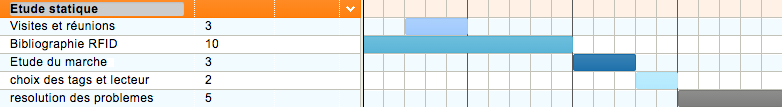
\includegraphics[width=\textwidth]{etudestatic}
\caption{Bibliographie et résolution des problèmes}

\end{figure}
\begin{figure}[H]
\centering
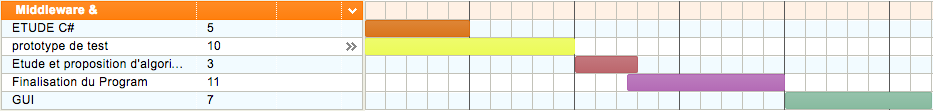
\includegraphics[width=\textwidth]{mid}
\caption{Middleware et interface graphique}

\end{figure}
\begin{figure}[H]
\centering
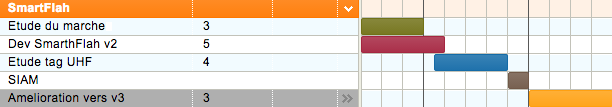
\includegraphics[width=\textwidth]{smart}
\caption{Développement de l'application SmartFlah}

\end{figure}
\begin{figure}[H]
\centering
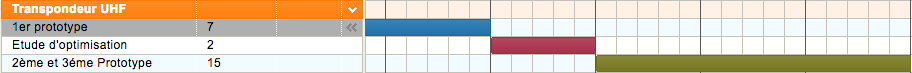
\includegraphics[width=\textwidth]{trans}
\caption{Conception du transporteur}

\end{figure}




\chapter{Généralité sur la technologie RFID}
RFID ou identification par fréquence radio, est une technologie en croissance rapide qui a le potentiel de faire de grands impacts économiques sur plusieurs industries. Bien que la RFID est une technologie relativement ancienne, les progrès les plus récents dans la technologie de fabrication de puces RFID font pratique à des nouvelles applications et paramètres.\\
Ce chapitre est dédié à l'étude	 détaillée de la solution RFID.
\section{Description de la solution}
Cette section présente les bases des systèmes RFID et offre la taxonomie des différents types de systèmes RFID. Nous discuterons brièvement deux normes RFID majeures et comment elles se rapportent à la pratique.
\subsection{Le système de base RFID}
La discussion de la technologie RFID a tendance à se concentrer uniquement sur les étiquettes. Il est plus exact de voir RFID comme un système complet qui comprend non seulement des étiquettes, mais aussi d'autres éléments importants. Les systèmes RFID sont constitués d'au moins trois composants principaux:
\begin{itemize}
\item Les étiquettes RFID ou transpondeurs, qui transportent les données d'identification.
\item Lecteurs RFID, ou des émetteurs-récepteurs qui permettent de lire et écrire des données dans l'étiquette.
\item Bases de données associés pour l'enregistrement des données d'identification\\
\end{itemize}

Nous illustrons l'interaction de ces composants dans la figure 3.1. Sur cette figure, trois étiquettes sont lisibles par un ou les deux lecteurs, A et B. Par exemple, l'étiquette 1 est lisible que par A, tandis que l'étiquette 2 est lisible par A et B, peut-être en raison de restrictions d'accès. Les lecteurs peuvent alors se connecter à des bases de données avec des enregistrements associés à des données d'identification. Dans ce cas, deux bases de données ont chacune son propre enregistrement.\\\\\\\\\\
\begin{figure}[!h]
\centering
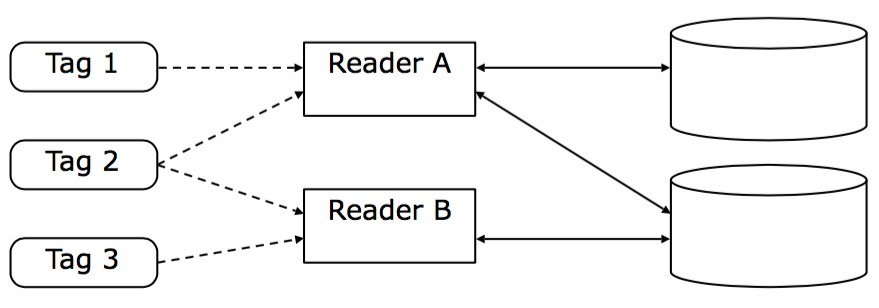
\includegraphics[width=\textwidth]{shema}
\caption{Illustration du système RFID}
\end{figure}
\subsection{Les composants essentiels d'un système RFID}
\subsubsection{Les tags}
Les tags sont attachés à tous les objets à identifier dans un système RFID. Un tag est généralement
composé d'une antenne et d'un circuit intégré. Une importante
distinction sera discutée plus tard sur la source d'alimentation d'un tag. Souvent, les étiquettes ne portent pas une source d'alimentation et doivent passivement récolter toute l'énergie nécessaire du signal RF \footnote{Radio Frequency}.\\

Il existe plusieurs types de tags qui offrent des différentes fonctionnalités et qui ont des puissances différentes
et ils fonctionnent à des fréquences radio différentes. Chacune de ces variables permet de déterminer
quelle application une étiquette particulière peut réaliser . Ces différences seront examinées plus loin dans ce chapitre.\\

Les étiquettes modernes ont tendance à mettre en œuvre la fonctionnalité d'identification sur un circuit intégré (IC) \footnote{Integrated Circuit} qui
assure le calcul et le stockage. Dans le procédé de fabrication, ce circuit intégré est fixé ou
"Attaché" à une antenne avant d'être emballée dans un facteur de forme, comme une capsule de verre ou une feuille, qui est intégrée dans le produit final. Dans la pratique, les différents fournisseurs effectuent souvent chacune de ces étapes de fabrication. Autres tags RFID peuvent être «chipless» ou avoir des informations d'identification lors de la fabrication, à savoir
"Écriture une fois, lecture nombreuse". \\
\begin{figure}[H]
\centering
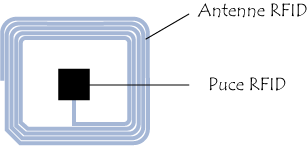
\includegraphics[height=3cm]{tag}
\caption{Tag RFID}
\end{figure}
\subsubsection{Reader ou Lecteur}
Les lecteurs RFID communiquent avec des tags à travers un canal RF pour obtenir l'identification
. Selon le type de l'étiquette, cette communication peut être un simple ping ou un protocole plus complexe de caractère multi-tour. Dans les environnements avec de nombreux points, un lecteur peut effectuer un algorithme d'anti-collision pour veiller à ce que les conflits ne se produisent pas. Les protocoles d'anti-collision permettent aux lecteurs de communiquer rapidement avec beaucoup de tags en série.\\

Les lecteurs alimentent souvent ce qu'on appelle des étiquettes passives à travers leur canal de communication RF.
Ces types d'étiquettes ne portent aucune puissance à bord et comptent uniquement sur un lecteur pour fonctionner. Ces tags sont si limités qu'ils comptent sur un lecteur pour effectuer des calculs.
Les lecteurs se présentent sous plusieurs formes, fonctionnent sur de nombreuses fréquences différentes, et peuvent offrir un large éventail de fonctionnalités. Les lecteurs peuvent avoir leur propre puissance de traitement et de stockage interne, et peuvent offrir une connectivité réseau. Les lecteurs peuvent être une simple conduite à un système externe, ou stocker toutes les données au niveau local.\\

À l'heure actuelle, de nombreuses applications reposent sur des dispositifs de lecture fixe. Les lecteurs RFID peuvent également être intégrés dans des appareils mobiles portatifs. Ces lecteurs mobiles permettraient à quelqu'un, par exemple, de faire l'inventaire d'un entrepôt en marchant à travers ses allées. Le fabricant de téléphone cellulaire Nokia propose déjà des fonctionnalités RFID de lecture dans certains de leurs téléphones cellulaires. Les tags de type EPC deviennent très réussi et intéressant . La fonctionnalité de lecture RFID pourrait devenir une caractéristique commune sur les téléphones, PDA \footnote{Personal Digital Assistant}, ou d'autres dispositifs informatiques portables cellulaires.
\begin{figure}[H]
\centering
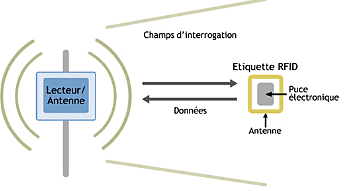
\includegraphics[height=4cm]{reader}
\caption{Interaction du Lecteur RFID avec son environnement}
\end{figure}
\subsubsection{La base de données}
Les bases de données RFID associent l'identifiant de tag avec un enregistrement qui peut contenir des informations sur les produits, les journaux de suivis, les données de ventes, ou les dates d'expiration. Des bases de données indépendantes peuvent être construites tout au long de la chaîne d'approvisionnement par des utilisateurs indépendants, ou peuvent être intégrés dans un système de base de données centralisé ou fédéré.\\

Les bases de données supposées avoir une connexion sécurisée aux lecteurs. Bien qu'il existe des scénarios où les lecteurs peuvent ne pas être dignes de confiance, il est souvent utile de faire écrouler les notions de lecteur et de base de données en une seule entité. Par exemple, si les étiquettes contiennent toutes les informations du produit en cause, il n'y a pas besoin de faire un appel à une base de données hors site.\\

On peut imaginer un système fédéré de bases de données back-end, où chaque fabricant de produit conserve son propre service de consultation. Dans ces paramètres, il peut être utile de déployer un ONS \footnote{Object Naming Service} pour localiser les bases de données associées à une valeur d'identification d'étiquette. Un ONS permet au lecteur de trouver un ensemble de bases de données associées à une valeur d'identification d'étiquette particulière. Ceci est analogue à l'Internet avec le DNS \footnote{Domain Naming Service} qui renvoie les adresses des serveurs qui peuvent traduire les noms de domaine en adresses IP \footnote{Internet Protocol} numériques. ONS n'a pas encore été largement adopté dans la pratique.
\subsection{Source d'énergie d'un Tag}
Comme brièvement mentionné précédemment, les étiquettes peuvent obtenir leur puissance d'alimentation de plusieurs manières différentes. La source d'énergie est une propriété essentielle d'une étiquette, car elle va déterminer la distance de lecture potentielle d'une balise, la durée de vie, le coût, et quel genre de fonctionnalités elle peut offrir. La source d'énergie sera également importante pour déterminer comment une étiquette peut être orienté et quelles formes physiques elle peut prendre. Il existe trois catégories principales de sources d'énergie d'un tag : actives, semi-passives, et passives.\\

 Les étiquettes actives ont leur propre source d'énergie, telle qu'une batterie, et peuvent initier une communication à un lecteur ou d'autres balises actives. Parce qu'elles contiennent leur propre source d'alimentation, les étiquettes actives ont généralement une plage de fonctionnement beaucoup plus large que passifs-tags. Une caractéristique clé de balises actives est qu'elles sont en mesure de lancer leur propre communication avec les lecteurs. Les balises actives avancées, pourraient même former des réseaux ad hoc les unes avec les autres. Une application utile des balises actives dans des conteneurs d'expédition , qui peuvent tomber hors navires sur les mers agitées. Ces conteneurs manquants parfois ne sont pas reconnus jusqu'à ce que le navire à quai . Une étiquette à puce avec un capteur accéléromètre peut détecter quand il est tombé et distribuer un journal de sa disparition avant de sombrer dans l'océan.\\

Par contre, une étiquette semi-passive (ou semi-active) a une batterie interne, mais n'est pas en mesure d'initier des communications. Cela garantit que les étiquettes semi-passives ne sont actives que lorsqu'elles sont interrogées par un lecteur. Parce que ces dernières ont une source d'énergie interne, elles offrent une lecture plus large que les passives, mais à un coût plus élevé.\\


Un exemple d'application qui utilise souvent des étiquettes semi-passives est \emph {tollbooths} électroniques. Les étiquettes sont généralement collées à l'intérieur du pare-brise d'une voiture. Lorsque la voiture passe par un péage, il lancera une requête à l'étiquette et lira le compte identifiant de l'étiquette. La batterie de bord permet à la balise d'être lue à une distance considérable. Cependant, étant donné que l'étiquette ne doit diffuser que lorsqu'elle est interrogée, elle peut rester inactive la plupart du temps et économiser de l'énergie. Les étiquettes semi-passives sont également souvent utilisées dans les palettes au niveau de suivi des composants tels que des pièces d'automobile lors de la fabrication.\\


Les étiquettes passives n'ont ni leur propre source d'énergie, ni la capacité d'initier la communication. Elles obtiennent de l'énergie par la récolte à partir d'un signal de communication RF entrant. À des fréquences plus basses, cette énergie est typiquement récoltée par induction, tandis qu'à des fréquences plus élevées, elle est récoltée par capacité.\\

Bien que les étiquettes passives ont la plus courte distance de lecture de tous les trois types , elles sont les moins chères à fabriquer et plus facile à intégrer dans les produits. Les batteries sont relativement coûteuses et ne peuvent pas facilement être incorporées dans certains articles, comme les emballages en papier. Pour cette raison, les étiquettes passives sont les balises les plus courantes.\\

En l'absence d'une source d'énergie interne dicte de nombreuses propriétés des étiquettes passives. D'abord, elles ne peuvent pas fonctionner sans la présence d'un lecteur, bien que l'étiquette passive pourrait temporairement emmagasiner  un peu d'énergie dans un condensateur. En raison de leur faible signal de réponse, les étiquettes passives sont souvent plus sensibles au bruit ambiant ou des interférences. Le tableau 1 compare diverses propriétés des étiquettes passives, semi-passives et actives.\\

\begin{longtable}{|p{0.35\textwidth}|p{0.2\textwidth}|p{0.2\textwidth}| p{0.15\textwidth}| p{0.15\textwidth}|}
\hline
\textbf{Type} & \textbf{Passif} & \textbf{Semi-Passif} & \textbf{Actif} \\
\hline
\textbf{Source d'énergie} & énergie récoltée du RF & Batterie & Batterie \\
\hline
\textbf{Communication} & Réponse seulement & Répondre seulement & Répondre et/ou initier \\
\hline
\textbf{Max Range} & 10 M & 100 M &  100 M \\
\hline
\textbf{Coût relatif} & Le moins cher & Plus cher & Très cher \\
\hline
\textbf{Exemple Applications} & EPC cartes de proximité & télé péage &  \emph {Livestock tracking} \\
\hline
\caption{Comparaison de tag passif , semi- passif et actif}
\end{longtable}


\subsection{Fréquences de fonctionnement}
Les systèmes RFID ont une variété de fréquences radio. Chaque bande de fréquences offre son propre avantage d'exploitation, les exigences de puissance et de performance. Différentes gammes peuvent être soumises à des règlements ou des restrictions qui limitent ce que les applications peuvent être utilisés pour.
Les métaux et les liquides présentent généralement le plus grand problème dans la pratique. En particulier, les balises actives dans l'ultra-haute fréquence (UHF) ne fonctionnent pas correctement à proximité des liquides ou des métaux.\\


La fréquence de fonctionnement est également importante dans la détermination des dimensions physiques d'une étiquette RFID. Différentes tailles et formes des antennes fonctionnent à des fréquences différentes. La fréquence de fonctionnement détermine également la possibilité d'interagir physiquement avec les autres. Par exemple, l'empilage des étiquettes plates feuille d'incrustation sur le dessus de l'autre peut interférer ou empêcher les balises de la lecture correctement. Le tableau 2 énumère les fréquences standards et leurs distances de lecture passives respectives.\\
\begin{longtable}{|p{0.35\textwidth}|p{0.2\textwidth}|p{0.2\textwidth}|}
\hline
\textbf{Gamme de fréquences} & \textbf{fréquences} & \textbf{Distance de lecture} \\
\hline
Basse fréquence & 120-140 KHz & 10-20 cm  \\
\hline
Haute Fréquence (HF) & 13,56 MHz & 10-20 cm \\
\hline
Ultra-haute fréquence (UHF) & 868-928 MHz & 3 mètres \\
\hline
Micro onde & 2,45 et 5,8 GHz & 3 mètres \\
\hline
Ultra-Wideband (UWB) & 3,1-10,6 GHz & 10 m \\
\hline
\caption{fréquences de fonctionnement RFID}
\end{longtable}
\subsubsection{Basse fréquence (LF)}
Les étiquettes RFID basse fréquence (LF) fonctionnent généralement dans la gamme 120-140 kilohertz. Plus souvent, les balises LF sont passivement alimentés par induction. En conséquence, elles ont généralement de très courtes intervalles de lecture 10-20 centimètres.\\

Les balises LF peuvent être utilisées dans des environnements difficiles et peuvent fonctionner à proximité de métal, des liquides, ou de la saleté. Cela les rend utiles pour des applications comme les étiquettes d'identification pour les animaux de compagnie implantables ou des étiquettes de gestion de blanchisserie. Un inconvénient de balises LF est son faible taux de lecture de données par rapport à d'autres fréquences de fonctionnement.\\

Les balises LF sont souvent utilisées dans les systèmes d'immobilisation de voiture et de contrôle d'accès. Dans ces systèmes, une voiture ne démarre que si une balise LF, généralement attaché à la clé de contact, est à proximité de l'allumage. Cela prend avantage de la courte portée de lecture de LF et l'utilise comme un élément de sécurité.\\

En 2016, les étiquettes LF passives peuvent être achetées à 10 DH par tag ou moins. Deux grands fabricants de balises LF sont Texas Instruments et Phillips Semiconductor. La norme \emph{ISO 18000-2 standard} \cite{iso2} offre des spécifications pour les étiquettes RFID LF.

\subsubsection{Haute fréquence}
Les étiquettes haute fréquence (HF) RFID fonctionnent à la fréquence de 13,56 MHz. Les étiquettes HF sont souvent emballées dans un facteur d'incrustation de feuille ou sous forme de carte de crédit. Cela rend les balises HF utiles pour la construction de contrôle d'accès, les cartes de crédit et des badges d'identification.\\

Les étiquettes HF sont également utilisées dans de nombreuses applications de suivi. Les bibliothèques et les librairies utilisent souvent un tag HF pour suivre les livres. Certains aéroports ont commencé à utiliser les étiquettes HF RFID pour les applications de manutention de bagages.\\

Les étiquettes HF offrent un taux de lecture de données plus élevé que les balises LF, mais ne réussissent pas aussi bien que les balises de LF à proximité de métaux ou de liquides. Cependant, elles offrent de meilleures performances à proximité de métaux ou de liquides que les tags UHF font.\\

La gamme de fréquences HF se trouve sur une partie fortement réglementée du spectre radio. Les signaux transmis par les lecteurs doivent fonctionner dans une bande de fréquences étroite. Cela pose un problème pour les environnements électroniques sensibles, tels que les équipements médicaux, qui fonctionnent sur des fréquences voisines. Cela rend les balises HF inappropriée pour les environnements comme les hôpitaux.\\

En 2016, les étiquettes HF passives peuvent être achetées à 5DH ou moins par étiquette. Texas Instruments et Phillips offrent deux lignes de tag HF, bien qu'il existe de nombreux fabricants plus petits et spécialisés ou intégrateurs dans l'espace de HF.
L'organisation internationale de normalisation (ISO) spécifie les étiquettes UHF par la norme \emph{ISO 18000-3 norme} \cite{iso}.\\
\subsubsection{Ultra-haute fréquence}
Les étiquettes Ultra-haute fréquence (UHF) RFID fonctionnent dans la gamme de 868 à 928 mégahertz. Les balises européennes fonctionnent généralement dans la gamme 868-870 MHz, tandis que dans les États-Unis et au Canada fonctionnent à 902-928 MHz. Les tags UHF sont les plus couramment utilisés pour les applications de suivi et de gestion de la chaîne logistique. Ceci est en grande partie parce qu'ils offrent une gamme à distance de lecture plus grande et sont moins chers à fabriquer que les tags LF ou HF . Les étiquettes EPC de première génération fonctionnent à des fréquences UHF.\\

Un inconvénient majeur des tags UHF est qu'ils éprouvent des interférences à proximité de liquides ou de métaux. De nombreuses applications telles que le suivi des animaux, suivi des conteneurs en métal, ou même de nombreux systèmes de contrôle d'accès sont irréalisables avec des étiquettes UHF. Certains matériaux ont été développés qui peuvent protéger les tags UHF de distorsion lié au métal, mais ceux-ci est loin à être utiliser dans la pratique. Les lecteurs UHF peuvent également interférer avec l'électronique sensible comme l'équipement médical.\\

Les tags UHF sont une technologie relativement récente que LF ou HF, et les coûts des lecteurs sont généralement plus élevés que les lecteurs de LF faible largeur de bande. En 2016, les tags UHF peuvent être achetés en quantités pour moins de 1DH par étiquette passive. Ces étiquettes UHF coûtes moins que  0.5DH sont susceptibles d'arriver sur le marché dans les prochaines années. Les étiquettes RFID fonctionnant à des fréquences UHF sont définies à la fois par l'ISO 18000-6 \cite{iso6} et la norme EPCGlobal \cite{air} .
\subsubsection{Micro-ondes} 
étiquettes de micro-ondes fonctionnent soit à 2,45 ou 5,8 GHz. Cette gamme de fréquences est parfois appelée la super-haute fréquence (SHF). La technologie RFID de micro-ondes est mise en usage assez récemment et se développe rapidement. Les étiquettes à micro-ondes utilisées dans la pratique sont généralement semi-passives ou actives, mais peuvent aussi se présenter sous forme passive. Les balises à micro-ondes semi-passives sont souvent utilisées dans l'identification de la flotte et des applications de télé-péage.\\


Les systèmes à micro-ondes offrent plus de taux de lecture que l'UHF. Les plages de lecture semi-passives et actives des systèmes de micro-ondes sont souvent plus grandes que leurs homologues UHF. Certains balises micro-ondes actives peuvent être lues à partir des distances allant jusqu'à 30 mètres, ce qui est moins comparé aux tags UHF . Cependant, les implémentations physiques des étiquettes micro-ondes  RFID peuvent être beaucoup plus petites et compactes que les étiquettes LF  RFID.\\


Il y a plusieurs inconvénients en ce qui concerne les balises à micro-ondes. La première est qu'elles consomment relativement plus d'énergie que leurs homologues de fréquence inférieure. Les étiquettes de micro-ondes sont généralement plus chères que les tags UHF. Commercialement parlant les balises actives disponibles coûtent autant que 250 DH par tag en 2016.
Un autre problème est que le sans fil 802.11b (WiFi) \cite{802.11b} peuvent interférer avec les systèmes micro-ondes RFID. Ainsi les dispositifs d'application de la ZigBee 802.15  \cite{802.15.4} prochaine norme sans fil pourraient potentiellement entrer en conflit avec des dispositifs micro-ondes RFID.
L'ISO 18000-4 \cite{iso4} offre des spécifications respectives pour les étiquettes RFID à 2,45 et 5,8 gigahertz. 
\subsubsection{Ultra-Wideband}
Ultra-wideband (UWB) appliqué à la RFID est assez récent. Plutôt que d'envoyer un signal fort sur une fréquence particulière, UWB utilise des signaux de faible puissance sur une très large gamme de fréquences. Le signal sur une fréquence particulière utilisée par UWB est très faible, mais dans l'ensemble, la communication est assez robuste. Dans la pratique, certaines implémentations de UWB fonctionnent de 3,1 à 10,6 GHz.\\

Les avantages de l'UWB sont qu'il a une très longue portée de lecture, peut atteindre 200 mètres dans certains contextes. UWB est également compatible avec le métal ou les liquides. Comme le signal sur une fréquence particulière est très faible, UWB n'interférer pas avec les équipements sensibles.\\

Un inconvénient d'implémentations actuelles de UWB est qu'il doit être actif ou au moins semi-passif. Cependant, étant donné que les balises UWB diffusent des signaux très faibles, ils sont relativement de faible consommation d'énergie. En 2006, il est difficile de savoir si la technologie existe pour créer un UWB tag passif.
La technologie RFID UWB est encore dans ses premières phases et il y a peu de produits disponibles dans le commerce. Les coûts de 50DH par tag sont raisonnables dans l'avenir proche .
\subsection{Fonctionnalité}
La fonctionnalité RFID de base est l'identification. Lorsqu'il est interrogé par un lecteur, les balises retournent un autre identificateur qui peut être utilisé pour récupérer d'autres enregistrements de données. Cependant, les étiquettes peuvent offrir d'autres fonctionnalités utiles dans différentes applications. Les principes et les technologies de ces différentes types de balises  sont si étroitement liées aux étiquettes RFID strictes, qu'elles sont souvent collectivement appelées «RFID». Bien qu'elles sont pas strictement RFID. Nous discutons de plusieurs classes majeures d'appareils liés à la RFID.\\

Nous avons partagé des étiquettes RFID en cinq grandes catégories: EAS, en lecture seule EPC, étiquettes de capteurs, et motes. Ceux-ci seront appelés classes A à E. EPCglobal propose cinq classes similaires de tag de la classe 0 à la classe 4 . Les classes EPCglobal alignées étroitement avec les notre, mais différentes quelque peu. Ces cinq classes sont résumées dans le tableau 3.3.

\begin{longtable}{|p{0.1\textwidth}|p{0.2\textwidth}|p{0.2\textwidth}| p{0.15\textwidth}|p{0.2\textwidth}|}
\hline
\textbf{Classe} & \textbf{Nom} & \textbf{Mémoire} & \textbf{Source d'énergie} & \textbf{Caractéristi-ques} \\
\hline
A & EAS & Aucun & Passive & article surveillance \\
\hline
B & Lecture seule EPC & Lecture seulement & Passive & identification seulement \\
\hline
C & EPC & Lire et écrire & Passive & Enregistrement de données \\
\hline
D & capteur Balises & Lire écrire & Semi-passive & capteurs environnementaux \\
\hline
E & motes & Lire écrire & active & Réseautage ad hoc \\
\hline
\caption{Classes de fonctionnalité des tags}
\end{longtable}

\subsection{Modes de transfert d’énergie et de communication}
Dans le premier cas (figure 3.4) . L’onde RF qui se propage de la station de base vers le tag n’a pour but unique que de fournir de l’énergie au tag de façon à charger la capacité d’alimentation afin que celle-ci puisse être capable d’alimenter l’ensemble du tag pour assurer son bon fonctionnement. Après cette phase d'alimentation, le tag est apte à recevoir des ordres de commande provenant de la station de base et de retourner des informations vers celle-ci. Puis le cycle recommence et il est à nouveau nécessaire de lui fournir de l'énergie pour continuer la communication et ainsi de suite. Bien évidemment, ceci prend du temps et manque parfois de souplesse.\\
\begin{figure}[H]
\centering
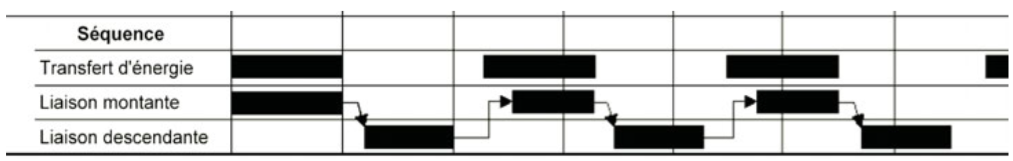
\includegraphics[width=\textwidth]{figa}
\caption{Mode de transfert d'énergie non simultané}
\end{figure}

Dans le deuxième cas (figure 3.5), au travers des principes et types de modulation utilisés, l'onde provenant de la station de base est capable pendant la phase de l'échange station de base vers tag d'assurer simultanément la fourniture de l'énergie et l'échange des informations (données).\\

\begin{figure}[H]
\centering
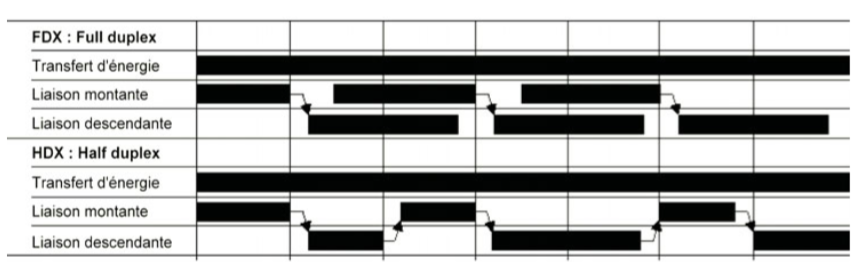
\includegraphics[width=\textwidth]{figb}
\caption{Mode de transfert d'énergie simultané}
\end{figure}

\begin{center}
\textbf{\emph{Note :}}\\
\emph{À noter que la très grande majorité des tags  en fonctionnement commercial sont basés sur ce dernier principe.}
\end{center}

\subsection{Liaison montante et liaison descendante}
Intéressons-nous d’abord aux échanges ayant lieu entre la station de base et les tags. Ils sont de deux types et seront définis  de la manière suivante :
\begin{itemize}
\item de la station de base vers le tag, dite liaison montante ;
\item du tag vers la station de base, dite liaison descendante. \\
\end{itemize}
De plus afin d’éviter quelques problèmes de compréhension, quelle que soit l’intelligence embarquée dans le tag, nous supposerons que celui-ci ne fonctionne que sous des ordres commandes provenant de la station de base. 
\subsubsection{Liaison montante ( forward link) de la station de base vers le tag}
La liaison montante (de la station de base vers le tag) a pour mission :
\begin{itemize}
\item d'assurer, si cela est possible, le transport de l'énergie vers le tag afin que celui-ci puisse assurer la tâche qui lui incombe ;
\item l'envoi de données de la station de base vers le tag ;
\item d'assurer, si cela est possible, le transport de l'énergie vers le tag afin que celui-ci puisse répondre
\item dans le cas des systèmes fonctionnant en mode passif (voir la définition), lors de la phase de communication en liaison descendante avant d'assurer la présence d'un support physique à la communication du tag vers la station de base.\\
\end{itemize}
La communication montante est par principe assurée par la station de base qui émet une onde radiofréquence. Celle-ci est donc dotée d’un émetteur et d'un transmetteur . De part la présence de cet émetteur, la liaison montante est dite active. De plus, la station de base comporte également à son bord un récepteur. La station de base est donc un transmetteur. Dans le sens montant, la station de base doit se faire comprendre par le tag au travers d’un codage numérique (binaire), d’un protocole de communication et d’un système de modulation de la fréquence porteuse qui ne doit pas ou peu affecter (le plus faiblement possible) la qualité des données. Pour cela on peut employer des techniques de modulation de fréquence FSK \footnote{Frequency-Shift Keying}, ou encore de nombreuses méthodes de modulation d’amplitude ASK \footnote{Amplitude-Shift Keying}
\subsubsection{Liaison descendante de la modulation}
Contrairement à ce qu'on pourrait initialement penser, le transpondeur ne peut pas se comporter comme un émetteur de signaux RF. En effet, il ne dispose pas, dans son interface RF, des mécanismes permettant d'émettre un signal radio-fréquence vers la station de base. Les transpondeurs utilisent ce qu'on appelle la réflexion d'ondes pour se faire comprendre par les lecteurs. \\

Pour cela, les tags utilisent une modulation différente que l'on nomme modulation de charge (Load Modulation) qui consiste à varier la charge résistive du circuit. Effectivement, en variant la charge, le tag varie l'intensité du courant dans son circuit et donc l'intensité qui circule dans l'antenne. La consommation d'énergie qu'il représente dans le champ magnétique est alors également modifiée et, par couplage magnétique, cela influence sur l'intensité du courant dans l'antenne de la station de base. De proche en proche, les signaux RF reçus de la station de base, qui sont réfléchis par le transpondeur, permettent donc de transporter des réponses en faisant varier l'intensité du circuit du lecteur.\\

Il s'agit ici d'un procédé assez complexe mais qui repose à la base sur de la modulation. Cette modulation de charge résistive à l'origine de la transmission de la réponse s'appuie sur une modulation courante appelée OOK \footnote{On Off Keying} et correspond à la modulation d'amplitude "tout ou rien". à l'aide d'une modulation de type OOK, comme présentée précédemment, on crée une modulation qui varie la charge résistive du circuit et donc la tension aux bornes du circuit RF du transpondeur comme montré dans la figure 3.5.\\
\chapter{Les solutions proposées et étude théorique }
Dans ce chapitre je vais présenter les trois projets qu'on a pu réaliser tout au long de ce stage, les solutions proposées et l'étude théorique . La première étape consiste à développer un middleware et un protocole de communication entre le lecteur et le client ,une base de données étant indisponible dans ce projet pour l'enregistrement des données. La deuxième étape consiste à réaliser une application Android pour la gestion des tags animal . Finalement la conception et la miniaturisation d'un transpondeur UHF.
\section{Client et interface RFID}

L'application desktop  est un logiciel pour la gestion des entrées et sorties des palettes du stock. Elle exécute au sein d'elle le protocole de communication qui à son tour communique avec le lecteur et le commande afin de bien gérer son interface air. Les détails de ce protocole sont décrites dans la section suivante. L'interface utilisateur permet une visualisation clair des données enregistrées, la gestion du serveur de base de données et les méthodes de sécurité de cette communication , les ajouts des dépendances comme l'état des palettes (in ou out).\\

Dans la figure suivante je présente l'architecture globale d'un système RFID. Notre interface se positionne entre le lecteur et la base de données. Cette interface permet l'acquisition des données du lecteur et les présenter sous une forme logique au utilisateur.

\begin{figure}[H]
\centering
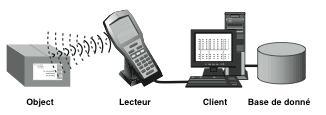
\includegraphics[width=9cm]{systemx}
\caption{Rappel du système RFID}
\end{figure}

\subsection{Étude du marché}
Le besoin concernant le produit étudié constitue un appel exigeant et irremplaçable, surtout pour les entreprises dont leur produit initial est livré dans des palettes ou des contenaires afin de garder sa qualité et faciliter la logistique . Ces palettes sont après rendues au fournisseur et dans des cas elles sont perdues, d'où la nécessité d'une solution optimale et automatique afin de garantir la traçabilité des palettes.

Notre solution propose une méthode simple et efficace pour une traçabilité claire et adéquate.
\subsection{\emph{Middleware} et Protocole de communication}
Le \emph{Middleware} est un protocole de couche application c'est un moyen d'échange logique entre le lecteur et le client. Il gère l'interface physique du périphérique ou il est exécuté. Il Contrôle l'initiation de la communication au serveur et la rupture de cette dernière. Dans la suite de cette section je vais décrire le rôle de ce protocole. Les responsabilités de cette interface sont les suivantes:
\begin{itemize}
\item Fournir des moyens pour commander un lecteur RFID  (lire les codes EPC sur les étiquettes), lire les étiquettes (lire d'autres données sur les étiquettes en dehors du code EPC), écrire dans les tags, et exécuter d'autres commandes d'accès du protocole dépendant.
\item 
Fournir un moyen de reporter l'état et la gestion des erreurs lors des opérations d'accès d'étiquette.
\item 
Fournir des moyens nécessaires pour effectuer des commandes qui peuvent en avoir besoin, comme la commande 'Kill' dans le Protocole UHF Interface Air \cite{air}.
\item 
Fournir des moyens pour contrôler les aspects du fonctionnement du protocole y compris les paramètres de ce dernier et les paramètres de signalisation.
\item 
Fournir des moyens pour faciliter l'ajout du support pour des nouveaux protocoles d'air
\item 
Fournir des moyens pour la récupération des capacités du lecteur.\\
\end{itemize}
\subsection{Rôle de l'interface}
L'infrastructure RFID est constituée des éléments de réseau qui participent à la gestion (par exemple, lecture / écriture / verrouillage) et la transmission des données de l'étiquette. Las destinations des données sont les éléments du réseau clients (applications par exemple, l'utilisateur final, base de données). Les éléments du réseau entre l'étiquette et les clients forment le support pour transporter les données de l'étiquette sur le réseau et de transmettre les commandes opérationnelles des balises.\\\\\\\\\\\\\\\\\\
\begin{figure}[H]
\centering
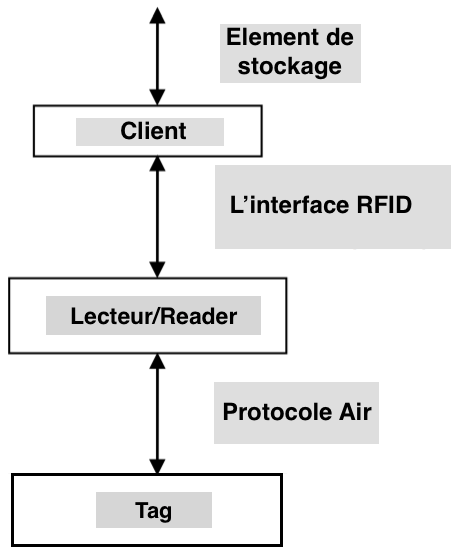
\includegraphics[width=6cm,height=8cm]{orga}
\caption{Emplacement de l'interface RFID}
\end{figure}

La figure 3.2 illustre la position de l'interface RFID dans l'architecture de la pile entre le rôle du client et le rôle du tag. Les rôles du client peuvent être classés en trois grands groupes fonctionnels: traitement des données d'étiquette, la gestion du lecteur et le contrôle du lecteur et de la coordination. Avec l'avènement des protocoles d'air sophistiqués comme UHF class 1 Gen-2 \cite{air}, et les déploiements du plus grand nombre de lecteurs, la nécessité d'un contrôle du lecteur et de la coordination  du réseau des lecteurs dans l'architecture devient importante.
Cette Interface facilite la fonction de contrôle en exposant le protocole d'air. En effet, cette interface est donc conçu pour être extensible en termes de support pour les protocoles d'air multiples.\\

Les exigences physiques et logiques pour la communication entre le lecteur et l'étiquette sont définies par le protocole de l'air. Plus précisément, le protocole d'air définit la couche de signalisation de la liaison de communication, les procédures et les commandes d'exploitation des lecteurs et étiquettes et l'arbitrage de collision comme schéma pour identifier une balise spécifique  dans un environnement multi-tag. La mémoire de l'étiquette dans le protocole C1G2 est logiquement divisée en quatre banques distinctes: la mémoire réservée, la mémoire de l'EPC, la mémoire TID et la mémoire utilisateur. La carte mémoire physique de l'étiquette est spécifique au fournisseur. Le protocole de l'air commande qui accèdent à la mémoire il a un paramètre qui sélectionne la banque, et un paramètre d'adresse pour sélectionner un emplacement de mémoire particulier au sein de cette banque.\\


Les opérations fondamentales d'un lecteur sur une population d'étiquette sont l'inventaire et l'accès. L'inventaire est l'opération  d'identification d'étiquettes. En utilisant le schéma d'anti-colision, le lecteur détecte une balise unique et demande le contenu de la mémoire de l'EPC de l'étiquette. L'accès est l'opération de communication avec (lecture et / ou écriture ) une balise. Une balise individuelle doit être identifié de manière unique avant l'accès. Semblable à l'opération d'inventaire, l'accès multiple comprend les commandes de protocole de l'air. En outre, un lecteur peut choisir un sous-ensemble de la balise de population pour l'inventaire et l'accès. Cette opération est appelée la sélection dans le protocole C1G2. L'opération de sélection est utilisée pour sélectionner et/ ou dé-sélectionner une population de balise particulière pour l'inventaire ultérieur et/ou opération d'accès. Cela permet de concentrer les opérations sur le sous-ensemble désiré de balises, et également la population d'étiquette participant à l'opération  d'anti-colision, améliorant ainsi le taux d'anti-colision globale.

Il est prévu que la performance globale du système peut être optimisée en réglant le RF, l'anti-colision et protocole d'air au sein et entre les lecteurs. La performance peut encore être optimisée si le réglage fait conscient de l'environnement RF dans le voisinage du Reader.\\
\subsection{Vue globale sur l'inerface RFID}
l'interface RFID concerne spécifiquement la fourniture des formats et des procédures de communication entre un client et un lecteur. Les unités de données de l'interface RFID sont appelés messages. Les messages du client vers le Reader permettent d'obtenir et définir la configuration des lecteurs, des capacités de découverte de lecteurs et de gérer les opérations d'inventaire et d'accès aux lecteurs. Les messages du Reader pour le client comprennent trois portions du statut Reader, enquête RF, l'inventaire et l'accès aux résultats. L'interface RFID est un protocole de couche d'application et ne fournit pas de retransmission, ou des installations de remise en ordre. La cohérence de l'état entre le client et le lecteur est essentielle pour le bon fonctionnement du système. En utilisant des messages , le client met à jour l'état du lecteur qui comprend ces paramètres de configuration, des structures de données crées dynamiquement et éventuellement des données des fournisseurs définis. Pour cette raison, le protocole exige des accusés de réception pour le client aux transactions Reader - cela fournit un mécanisme de sécurité à la couche application pour faire face à des situations d'erreur réseau. En outre, pour faire face à des connexions intermittentes, un client peut demander l'état de configuration d'un lecteur pour confirmer que l'état d'un lecteur est compatible avec le client. Les messages des clients sont principalement des rapports, des notifications d'état ou keepalives. Seuls les keepalives sont reconnus par le Client.
\begin{figure}[!h]
\centering
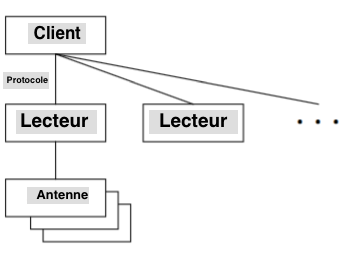
\includegraphics[width=6cm,height=6cm]{lim}
\caption{Illustration du système RFID}
\end{figure}
Comme on le voit sur la figure 3.7, du point de vue de notre protocole, un lecteur contient une collection d'une ou plusieurs antennes. De plus, les lecteurs employés présents dans le cahier des charges ne sont pas nécessairement en correspondance un à un avec les dispositifs matériels.
\subsection{Chronologie de fonctionnement du protocole}
Le fonctionnement du protocole ou d'une connexion comporte deux phases: la phase de négociation et la phase exécution.
\subsubsection{Phase de négociation}
Un client et un lecteur devront négocier une version de protocole pris en charge mutuellement pour chaque connexion. Lorsqu'une connexion  est d'abord établie, à la fois le client et le Reader supposent la version 1. A l'exception des messages de négociation de version, les messages sont envoyés par le client  jusqu'à ce que le processus de négociation de version est complet. La négociation de la version est effectuée en utilisant des messages prédéfinis et initiés par le client. Le client demande la version de protocole pris en charge par le Reader, puis détermine une version appropriée pour la connexion (type de message).
 
Une fois qu'une version a été établie à l'aide de cette procédure, tous les messages qui suivent sont envoyés en utilisant les messages prédéfinis par le lecteur. La chronologie du fonctionnement de la phase de négociation  entre un client et un lecteur est représentée sur la figure 3.4.
\begin{figure}[!h]
\centering
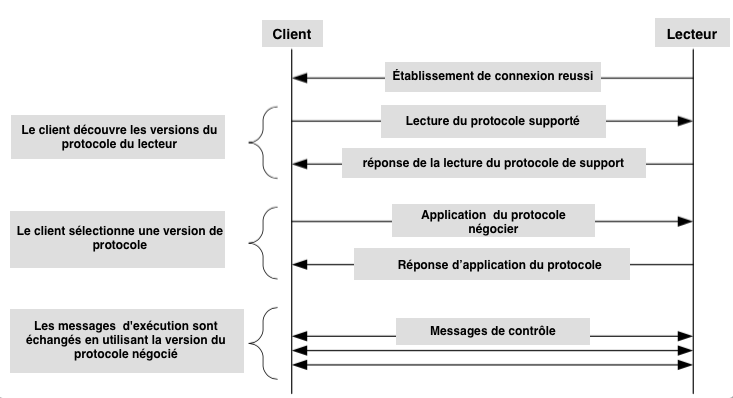
\includegraphics[width=\textwidth]{negotiation2}
\caption{Phase de négociation}
\end{figure}
\subsubsection{Phase d'exécution}
L'opération d'exécution comprend les phases suivantes:
\begin{itemize}
\item Découverte des capacités
\item Configuration de l'appareil
\item Opérations d'inventaire et d'accès aux cycles de configuration d'inventaires exécutés
\item Si les conditions d'étiquettes sont adaptées, les opérations d'accès seront exécutées pendant l'exécution du cycle des stocks.
\item Les opérations d'accès incluent la lecture, l'écriture et de verrouillage du mémoire d'étiquette, étiquettes tuant, etc.
\item Les opérations RF
\item Rapports retournés au client
\end{itemize}

La figure 3.5 illustre toutes les étape des messages échangés entre le lecteur, client et les tags.

Le protocole utilise des unités des données appelées messages pour communiquer entre le client et le Reader pour les mises à jour des clients ou pour récupérer la configuration du lecteur, en générale pour le contrôle du fonctionnement du lecteur. Cette section nous a donné un aperçu globale du modèle abstrait du protocole, dans le chapitre suivant on va présenter le logiciel qui met en œuvre ce protocole.
\begin{figure}[!h]
\centering
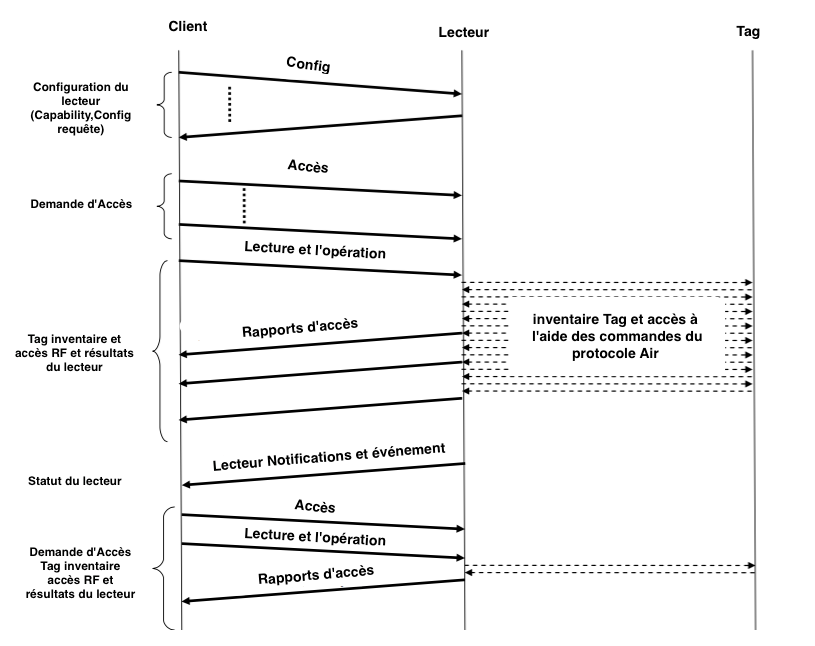
\includegraphics[height=12cm]{runtime}
\caption{Phase d'exécution}
\end{figure}
\pagebreak





\section{SmartFlah}
%describe everything you did in The Android
Dans cette section on va parler du dernier projet qui consiste à développer une application Android pour le tag LF. On va commencer par une petite présentation du plate-forme Android puis on va parler de toutes les fonctionnalités que l'application nous permet de faire. Aussi une étude sur le domaine d'agriculture qui nous a inspiré à réaliser ce projet .\\
\subsection{La plate-forme Android}
Android est le logiciel qui fait tourner plus d’un téléphone ou tablette dans le monde.
Il est de type système d’exploitation mobile comme « Windows » est un système d’exploitation sur PC.Il fait tourner votre mobile. Il existe d’autres systèmes d’exploitation mobile concurrents comme iOS Apple, BlackBerry OS, Bada, Windows mobile… il est ouvert donc le code source est librement accessible (contrairement aux systèmes de Apple ou Microsoft) ce qui permet à n’importe quel fabricant de l’intégrer dans son système gratuitement. Ce modèle est opposé au modèle d'Apple, et explique en grande partie la forte croissance. Android est basé sur Linux qui tourne sur une grande variété de marques de téléphones et de tablettes différentes telles que Samsung, Motorola, Sony, Google Nexus, Acer, LG, Dell et bien plus encore (liste complète sur android.com) Cette diversité représente à la fois un avantage (diversité et choix pour le consommateur) et un inconvénient (problèmes de compatibilité des applications avec les différents modèles, en particulier les plus exotiques)
\subsection{Étude du marché de l'agriculture}
La majorité des éleveurs au Maroc, que ça soit dans l'élevage pour la production ou pour l'amélioration d'une race, ont un besoin urgent pour des solutions de gestion de leur production ou leur stock. Avec la convention que l'état a lancé qui consiste à mettre un tag LF dans les oreilles des bêtes. Le rêve des éleveurs pour des solutions statistiques qui vont les aider à améliorer leur production ou de détecter les points faibles dans leur manière de gérer leur ferme est devenu indispensable. L'état n'a pas présenté une solution informatique au éleveurs, il a juste installé les tags et affecté les ID au éleveurs pour la sécurité, mais ce n'était pas assez intéressant pour l’éleveur qui ne veut qu'avoir le maximum d'information concernant sa ferme.\\

Ici on montre un besoin énorme pour une solution qui informatise notre domaine de production agricole que ça soit la production du viande rouge ou du lait. C'est pour cela, avec le soutien de MASciR, on a pu concevoir un prototype d'une solution informatique pour les éleveurs marocains. Dans ce qui suit je vais faire une présentation globale de notre solution.

\subsection{La conception de la base de données}
Tout project informatique se base énormément sur une base de données puissante, ce qui fait appel à la conception de notre base de données qui se divise en trois étape indispensable.
.
\begin{itemize}
\item Analyse de la situation existante et des besoins
\item Création d'une série de modèles conceptuels (canonique et vues externes) qui permettent de représenter tous les aspects importants du problème
\item Implémentation d'une base de données dans un SGBD, à partir du modèle logique

\end{itemize}

\begin{figure}[H]
\centering
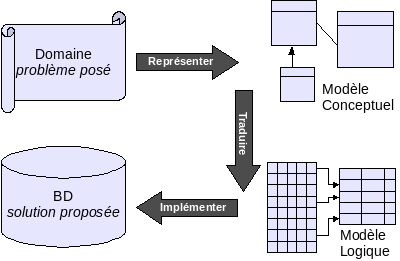
\includegraphics[width=8cm]{db}
\caption{Étape de conception d'une base de données}
\end{figure}

\subsubsection{Cycle d'abstraction de conception des systèmes d'information}
La conception du système d'information se fait par étapes, afin d'aboutir à un système d'information fonctionnel reflétant une réalité physique. Il s'agit donc de valider chacune des étapes en prenant en compte les résultats de la phase précédente. D'autre part, les données étant séparées des traitements, il faut vérifier la concordance entre les données et traitements afin de vérifier que toutes les données nécessaires aux traitements sont présentes et qu'il n'y a pas de données superflues.\\
Cette succession d'étapes est appelée cycle d'abstraction pour la conception des systèmes d'information :

L'expression des besoins aboutit au MCC (Modèle conceptuel de la communication) qui définit les flux d'informations à prendre en compte.
L'étape suivante consiste à mettre au point le MCD (Modèle conceptuel des données) et le MCT (Modèle conceptuel des traitements) décrivant les règles et les contraintes à prendre en compte.
Le modèle organisationnel consiste à définir le MLD (Modèle logique des données) qui représente un choix logiciel pour le système d'information et le MOT (Modèle organisationnel des traitements) décrivant les contraintes dues à l'environnement (organisationnel, spatial et temporel).
Enfin, le modèle physique reflète un choix matériel pour le système d'information. 


\begin{longtable}{|p{0.2\textwidth}|p{0.2\textwidth}|p{0.2\textwidth}| p{0.2\textwidth}|}
\hline
\textbf{Niveau } & \textbf{Statique (données) } & \textbf{Dynamique (traitements) } & \\
\hline
Conceptuel  & MCD & MCT  & Indépendant du système \\
\hline
Organisationnel ou logique  & MLD & MOT & Choix du SGBD
 \\
\hline
Opérationnel
ou physique  & MPD  & MOPT  & Haute connaissance du
SGBD \\
\hline
\caption{Cycle d'abstraction d'un système d'information}
\end{longtable}

Notre conception pour cette solution résulte en trois tables (tag,vaccin,docteur). Chaque tag représente un animal et chaque animal a une date de naissance, une race, un propriétaire et bien sûr pour des contraintes informatique on a été obligé d'ajouter des informations supplémentaire comme l'altitude la longitude et la date quand le tag a été lu.

Un animal doit faire d'une maniéré périodique des vaccins chez un docteur. Pour des raisons informatique on a ajouté des champs comme type de vaccin et la remarque. Bien sûr pour identifier un docteur on a besoin de son nom et son adresse. Ces attribues seront utilisés ultérieurement pour la conception et la gestion des informations.

\begin{figure}[!h]
\centering
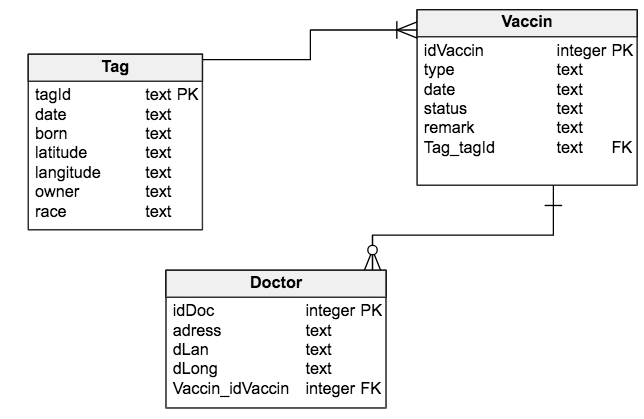
\includegraphics[width=10cm,height=9cm]{ddb}
\caption{Modèle de base de données}
\end{figure}

\subsection{Fonctionnalité}
L'application nous permet de lire l'identifiant du tag LF, cette étape consiste à faire un décodage du langage compris par le téléphone et ce qu'on a utilisé comme donnée au niveau de notre base de données et traitement de l'information. Après cette étape deux scénarios se manifestent soit le tag est déjà dans notre base de données et dans ce cas on offre à utilisateur la possibilité de consulter les données relier à son ID en parallèle l' application nous permet de visualiser l'historique de toutes les lectures effectuées. L'autre scénario c'est celui ou le tag n'a jamais été dans notre base de données, dans ce cas on demande à utilisateur de remplir des informations reliées à l'animal et bien sûr une autre possibilité est celle de remplir les informations dans le cas ou le docteur consulte l'animal. Finalement l'application permet de sauvegarder les données en générant un rapport automatique au serveur.

\begin{figure}[H]
\centering
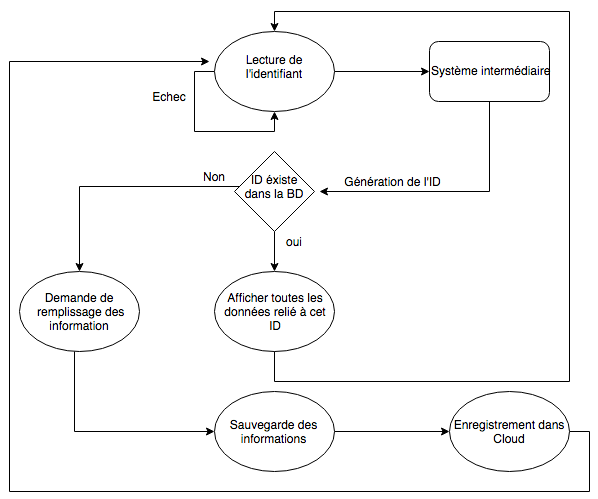
\includegraphics[width=10cm,height=9cm]{fonc}
\caption{Fonctionnalité de l'application}
\end{figure}
Les tests et vérification seront présentés dans le chapitre suivant ainsi que les captures et l'explication de l'interface d'utilisateur.

\section{Antenne UHF}
RFID a de nombreuses applications, une utilisation de cette technologie est pour l'identification des objets dans un stock. Les objets tels que les palettes et les cartons sont étiquetés de façon à lutter contre, le vole et la mauvaise gestion du stock. La détection des objets encapsulés dans les cartons était une tâche impossible sans ouverture des cartons, maintenant avec la RFID cette tâche et devenue une question de quelques secondes.
\subsection{Introduction}
Les étiquettes RFID utilisées auparavant pour cette application sont passives et surtout opèrent dans la basse fréquence (LF). Cependant, les balises LF ne peuvent être lues qu'a courte portée et peuvent ne pas bien se comporter lorsque plusieurs balises sont simultanément présentes dans le domaine. Les solutions se tournent maintenant vers l'utilisation des tags UHF. Les tags UHF non seulement donnent une meilleur distance de lecture, mais prennent également en charge des débits plus élevés. \\

Dans cette section, je vais présenter  une étiquette RFID passive qui opère dans la fréquence de 915MHz (UHF) . Dans la section suivante, une bref  théorie  sur l'antenne de l'étiquette et la puce utilisées dans notre conception, ainsi que la topologie de la conception théorique et pratique utilisée, suivie d'une discussion sur les points forts de la conception et des détails de sa mise en œuvre pratique avant que les conclusions ne soient présentées dans la dernière section.
\subsection{Antenne à boucle circulaire et puce alien}
L'antenne choisie pour l'étiquette est une antenne en boucle. La figure 3.9 montre une antenne en boucle ayant un diamètre D de la boucle et un fil de diamètre d. Une antenne en boucle est choisie car elle dispose d'une structure circulaire qui permet de minimiser la taille par rapport aux autres technologies comme les middreddeds et les Microstrips.\\

Une antenne à dipôle électrique est non plus possible. Pour la fréquence de fonctionnement qu'on utilise le problème du dipôle électrique à demi-onde sera sa grande taille cependant un petit dipôle peut être utilisé, mais l'expérience a montré qu'il est difficile de l'adapter.
\begin{figure}[H]
\centering
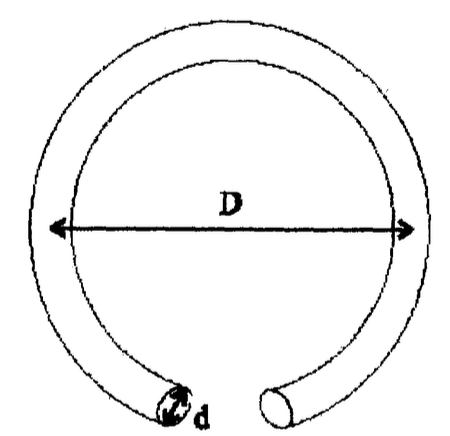
\includegraphics[width=4cm]{cla}
\caption{Antenne filaire}
\end{figure}

Le circuit équivalent de l'antenne est tel que représenté sur la Figure 3.10 a. En se référant à ce circuit, Rr est la résistance de rayonnement de l'antenne alors que L est son inductance. Dans l'hypothèse du flux uniforme du courant, R de notre antenne  peut être calculée en utilisant l'expression \cite{antennatheory}:

\begin{equation}
R_{r}  = 20 (\pi)^{2}(\beta a)^{4}
\end{equation}
Sur l'hypothèse des courants circulant sur la surface, l'inductance L de l'antenne peut être calculée en utilisant l'expression suivante \cite{antennatheory}:
\begin{equation}
L  = \frac{\mu_{0}D}{2}[ln(\frac{8D}{d})-2]
\end{equation}

Dans la figue 3.10 b le circuit équivalent de la puce RFID, qui peut être représenté par une résistance R et un condensateur  C en parallèle . R et C utilisés dans l'analyse et la conception de l'étiquette sont respectivement 1.5 k\(\Omega\) et 0.85 pF .

\begin{figure}[H]
\centering
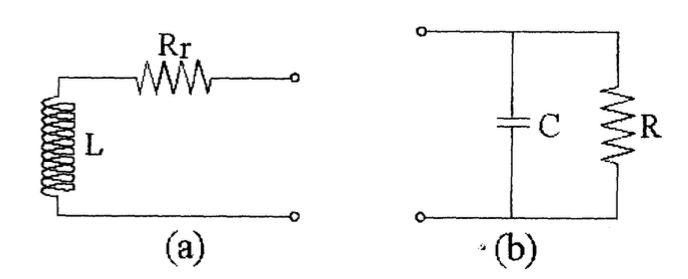
\includegraphics[width=8cm]{eq}
\caption{(a) le circuit équivalent pour une antenne en boucle; (b) RFID tag puce}
\end{figure}

\subsection{Design du Tag}
La fréquence de fonctionnement de l'étiquette se trouve dans la bande UHF.
La fréquence de 915 MHz a été choisie. Dans la conception initiale, le diamètre de l'antenne en boucle a été d'environ 2,2 cm avec un fil rond de 0.2 cm de diamètre  (D = 2.2cm d = 0.2cm).

En se référant à la figure 3.10 a et se référant aux équations (3.1) et (3.2), la résistance de rayonnement R de l'antenne en boucle peut être calculée pour être de 0,39  \(\Omega\) et la valeur de l'inductance L pour être  34,24 nH.\\

Le circuit RC équivalent de la puce RFID, comme représenté sur la Figure 3.10 b peut être transformé en circuit équivalent en série constitué d'une résistance  R' et une capacité C'. Les valeurs R' et C'  peuvent être calculées à environ 17.36 \(\Omega\) et 1,17 pF respectivement sur la base des valeurs R et C indiqué ci-dessus.\\


Par conséquent, à 915 MHz, l'impédance de source \(Z_{antenne} \) est de 0,39 ± j199 \(\Omega\) tandis que l'impédance de charge \(Z_{charge} \) est 17.36-j149.2 \(\Omega\). On sait que le transfert de puissance maximale se produit lorsque l'impédance de source est égale au conjugué de l'impédance de charge. Par conséquent, un réseau d'adaptation est nécessaire pour obtenir un transfert de puissance raisonnable.\\

Il existe trois réseaux d'adaptations de base utilisés dans les conceptions RF sont \emph{L-shape}, \(\Pi\) et la configuration T. Chacun d'eux a ses avantages et ses inconvénients. Le réseau d'adaptation le plus couramment utilisé est \emph{L-shape} . Les raisons sont les suivantes:
\begin{itemize}
\item Simplicité - Facile à construire des réseaux d'adaptation automatique. Il n'a que deux éléments à contrôler pour ajuster la partie réelle et imaginaire de l'impédance.
\item valeurs de composants pratiques - certaines des configurations nécessitent sois des valeurs d'inductance très basses ou très hautes valeurs de capacité ce qui est impossible à réaliser surtout quand vous devez concevoir un réseau d'adaptation automatique avec une gamme très large.\\
\end{itemize}

Le facteur de qualité Q du circuit est déterminé uniquement à partir de la source (générateur) et la charge (impédance du Circuit d'impédance) et ne dépend pas des composants externes - ce qui est peut-être la propriété la plus importante du circuit. Cela signifie que pour certaine impédances de charges il n'y a pas qu'une combinaison de L et C correspondante à cette charge.
\begin{equation}
Q = \sqrt{\dfrac{R_{source}}{R_{charge}}-1}
\end{equation}

Maintenant, en utilisant la définition de Q à vide pour trouver les branches en séries et en parallèles .
\begin{equation}
X_{1}=QR_{source}
\end{equation}
\begin{equation}
X_{2}=\dfrac{R_{p}}{Q}
\end{equation}

Le réseau d'adaptation T et \(\Pi\) nécessitent un algorithme de contrôle plus complexe pour la conception automatique du réseau d'adaptation. Il nécessite le contrôle de trois composants qui le rend plus cher. L'inconvénient du circuit en L est qu'il peut correspondre qu'aux charges égale ou inférieure à 50 Ohm. Si le circuit de L est inversé, il ne peut correspondre qu'à des charges égale ou supérieure à 50 Ohm. Il ne peut pas correspondre aux deux côtés. Par exemple, si la charge est entrain de se changer de 35 à 100 ohms, le réseau en L inversé correspond uniquement à partir de 50 à 100 ohms et ne correspondra pas à 35-50 ohms.
\begin{figure}[H]
\centering
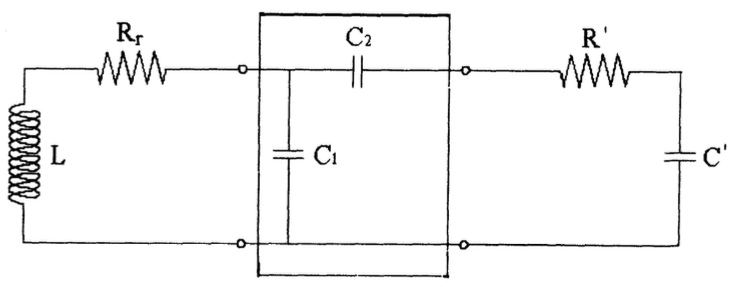
\includegraphics[width=8cm]{matcha}
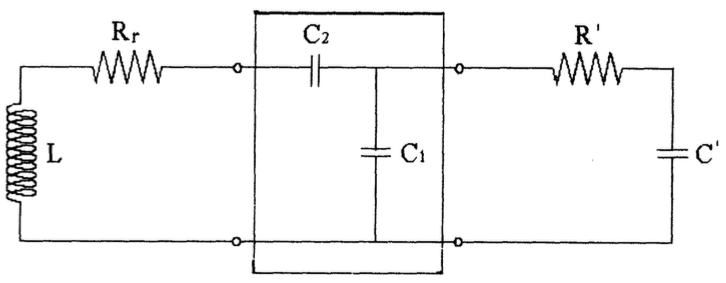
\includegraphics[width=8cm]{matchb}
\caption{Circuit d'adaptation L-shape}
\end{figure}
La figures 3.11 montre deux différents réseaux d'adaptation qui sont utilisés dans notre design. C1 et C2 peuvent être calculés numériquement ou en utilisant \emph {Smith Chart}. Les valeurs calculées de C1 et C2 pour ces deux topologies que nous considérions sont présentés dans le tableau 3.2.\\
\begin{longtable}[c]{| c | c | c |}
 \hline
  & Figure 3.8a & Figure 3.8b\\
 \hline
 \(C_{1}\) / pF & 0.743 pF & 6.557 pF\\
 \hline
 \(C_{2}\) / pF & 0.148 pF & 0.998 pF\\
 \hline
\caption{Réseau d'adaptation}
\end{longtable}
\subsection{Conception de mise en œuvre pratique}
La conception a été démarré à l'aide d'une antenne en boucle et un réseau d'adaptation conçu comme indiqué dans les sections précédentes. L'étape suivante consiste à examiner la mise en œuvre pratique de l'étiquette. Il a été décidé de mettre en œuvre la conception sur une très mince substrat avec une couche de cuivre sur l'avant côtés. La vue d'arrière du produit final est montrée dans la conception figure 3.12. En utilisant le réseau d'adaptation représenté dans la figure. 3.10 b. Cela ne signifie pas que le réseau d'adaptation représenté sur la figure 3.10 a est meilleur que l'autre. Les deux réseaux d'adaptation sont équivalents à la fréquence de résonance, les raisons pour lesquelles l'une représentée sur la figure 3.10 b a été choisi était parce qu'elle est plus facile à mettre en œuvre par la méthode utilisée ici.\\\\
\begin{figure}[H]
\centering
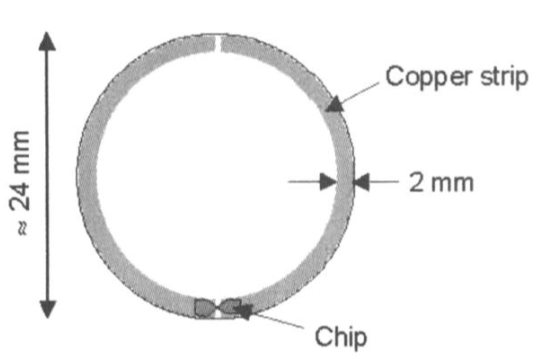
\includegraphics[width=6cm]{front}
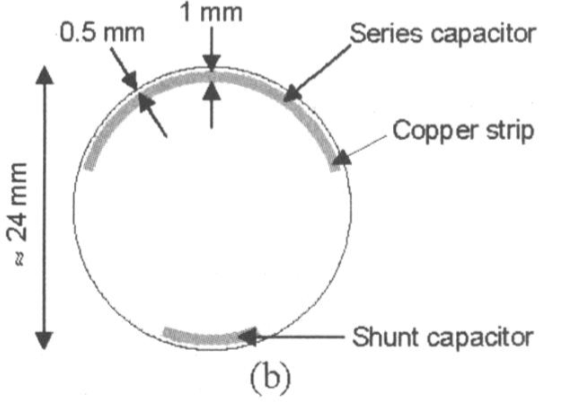
\includegraphics[width=6cm]{back}
\caption{Antenne à loup circulaire}
\end{figure}

Cette conception UHF de tag est constituée d'une antenne de boucle circulaire avec un réseau d'adaptation à deux éléments pour correspondre les impédances de l'antenne de l'étiquette et de la puce. Cependant, l'étiquette a été rendue légèrement plus grande en diamètre par rapport à celui présenté dans la figure 3.12 en fonction de l'application étudiée. 

Notre conception UHF d'étiquette dans la figure 3.13 considérée est constituée d'une antenne à dipôle électrique avec une piste de courbe d'inductance à travers le dipôle à des fins d'adaptation d'impédance. La structure et les dimensions de cette balise sont représentés sur la figure 3.13. Cette balise est faite en utilisant une carte FR4 avec une épaisseur de substrat h = 1,6 mm et de permittivité diélectrique \(\epsilon_{r}\) = 4,4. Cette conception de l'étiquette est de simple face.

 La structure d'antenne est simulée en utilisant CST studio 2014 et l'impédance simulée est de 20 + j152 \(\Omega\). Comme on peut le voir, l'impédance de la structure d'antenne de l'étiquette n'est pas exactement le conjugué de l'impédance de la puce \cite{alien} et donc, l'étiquette et l'impédance de la puce ne sont pas tout à fait adaptées.
\begin{figure}[H]
\centering
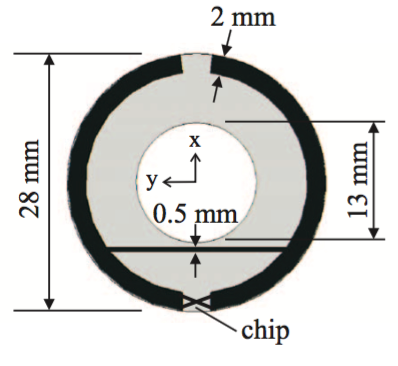
\includegraphics[width=6cm]{dofi}
\caption{Antenne à inductance}
\end{figure}

Cependant, la piste d'inductance à travers le dipôle ne fournit pas d'inductance suffisante pour accorder à la capacité de la puce de l'étiquette. Le diagramme de rayonnement de l'antenne, avec un maximum de directivité de 1,83 dB. Comme on le voit sur la section de simulation, bien que la forme générale du motif de rayonnement du première et seconde étiquettes UHF est presque identique, la directivité maximale de ces deux balises se produisent à différentes directions par rapport au plan des étiquettes. Les deux tags UHF ne sont pas testés et les résultats théoriques de la distance de lecture sont présentés dans le tableau 3.3.\\

\begin{longtable}[c]{| c | c | c |}
 \hline
  & UHF tag 1 & UHF tag 2 \\
 \hline
 Tag dans l'espace libre & 1.00 & 0.48\\
 \hline
 Tag attaché à la main  & 0.20 & 0.27\\
 \hline
\caption{Distance de lecture}
\end{longtable}
\subsection{Miniaturisation des antennes CLA}
Le cahier de charge impose par la nature de la solution à concevoir une antenne de petite taille (<2cm), la radiation doit être dans la bande autorisée par l'ANRT et la puissance reçu au niveau de la puce doit être suffisante pour alimenter le circuit. Les deux antennes précédemment présentés ont une taille relativement grande et les résultats de la simulation prédisent une mauvaise alimentation du circuit de la puce. Donc on a été obligé de penser à une solution pour réduire la taille et améliorer les performance de l'antenne. La littérature \cite{stub}  propose une solution possible qui peut
miniaturiser une antenne en boucle circulaire (CLA) à l'aide de \emph{short stubs} insérés dans la partie interne de la boucle. Dans le cas d'une longueur d'onde et une demi-longueur d'onde, respectivement, l'antenne est réduite jusqu'à 83\% et 92,1\% de sa taille par rapport au type CLA général. Par ailleurs la perte de retour, la bande passante -10dB et le gain d'une longueur d'onde et une demi-longueur d'onde sont respectivement de 12MHz (1,3\%), et de 48MHz (5\%). La deuxième méthode sera présentée avec la partie simulation dans le chapitre suivant.\\

La figure 3.14 présente des caractéristiques de changement de fréquence de résonance lorsqu'un \emph{short stubs} est mis en œuvre à l'intérieur de la boucle de l'antenne. La longueur du  \emph{short stubs} est de 20 mm et la fréquence de résonance chute 30MHz (3,3\%) à partir de 911.25MHz à 881.25MHz lorsque l'écart de la ligne est 2mm. En effet, le courant est distribué tout au long de la longueur totale de la boucle est augmentée à 13\%. En outre, non seulement les capacités sont augmentées par la dilatation de la longueur de la boucle, mais aussi les inductances sont augmentées par la structure de \emph{short stubs}. Par conséquent, l'impédance de l'antenne permet une adaptation d'impédance que la longueur de boucle est supérieure à une longueur d'onde,de sorte que la fréquence est éventuellement diminuée. Si elle est résonante à la même fréquence, le diamètre total de la boucle devient plus petit, de sorte que le cadre l'antenne est miniaturisé par les bouts des joints.


\begin{figure}[H]
\centering
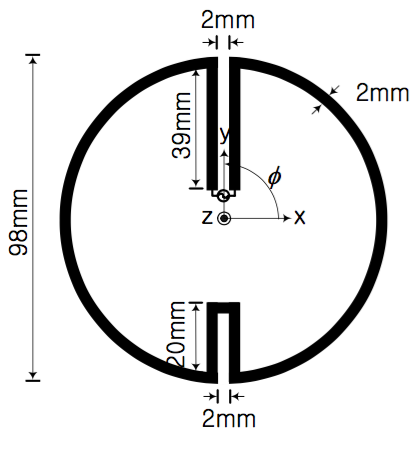
\includegraphics[width=4cm, height=4cm]{stuba}
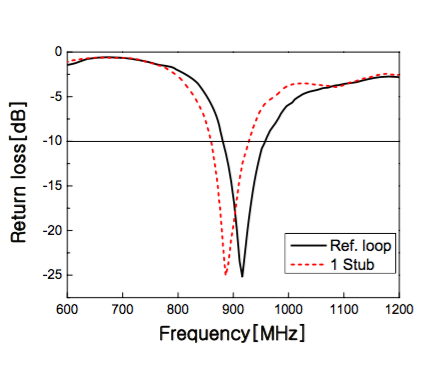
\includegraphics[width=4cm, height=4cm]{stubb}
\caption{La variation du S11 après l'ajout du stub}
\end{figure}

\begin{figure}[H]
\centering
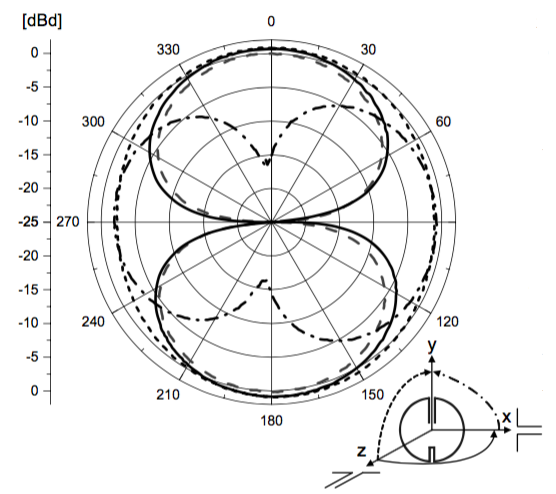
\includegraphics[width=5cm]{lob}
\caption{far-field pattern de l'antenne avec stub}
\end{figure}

Au moyen du procédé de miniaturisation de l'antenne en boucle, l'antenne de la figure 3.16 est miniaturisé avec des \emph{short stubs} de 11,5 mm et 7 mm . La largeur de la ligne est de 0.3mm et l'intervalle entre les lignes est de 0.3mm
Il est adapté à la longueur et l'intervalle de la ligne d'alimentation qui est de 8mm et 1mm. Le diamètre d'une antenne est miniaturisé à 40 mm.\\
\begin{figure}[H]
\centering
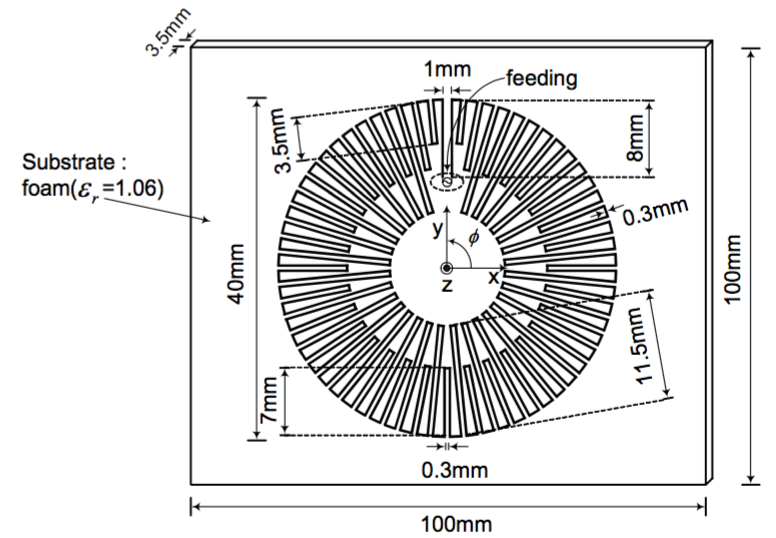
\includegraphics[width=6cm]{structure}
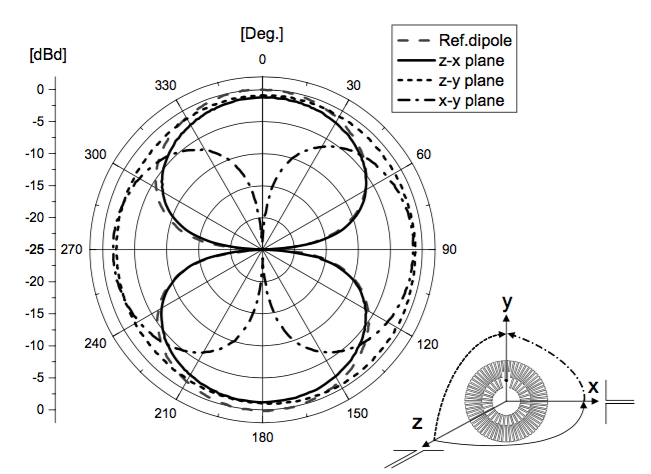
\includegraphics[width=6cm]{structurea}
\caption{CLA après miniaturisation}
\end{figure}

Une autre méthode a été conçu après des expériences de \emph{Reverse Engineering} des tags UHF achetés du marché. Cette méthode consiste à boucler l'antenne en interne de tel sorte à minimiser le diamètre sans changer la longueur des deux pôles. La figure suivante présente les résultats de l'analyse par  \emph{X-RAY Reverse engineering} qui permet de voire en interne sans massacrer la pièce. La figure suivante présente les résultats du \emph{Reverse engineering}. L'étiquète est constituée de deux couches de cuivre, la puce est fixée sur l'antenne le fixage est avec \emph{wire bonding}. La simulation de cette antenne sera présentée dans le chapitre suivant. \\\\\\\\\\\\\\\\

\begin{figure}[H]
\centering
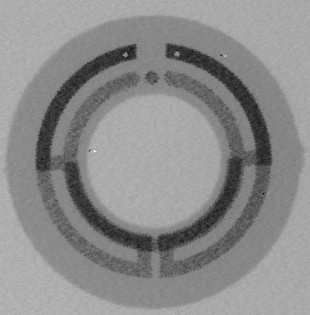
\includegraphics[width=5cm]{xray}
\caption{X-Ray du tag UHF}
\end{figure}

On s'est inspiré de cette méthode, qu'on appellera dans ce rapport \emph{bouclage interne} pour améliorer notre antenne et l'optimiser au niveau de la taille. La figure suivante montre la nouvelle version de l'antenne en figure 3.18. La taille a été réduite de 30 \% on a passé de 28 mm à 22 mm. La nouvelle structure permet un contrôle facile de fréquence et d'impédance. Dans les sections qui suivent on présente une étude détaillée sur les avantages de cette nouvelle structure et aussi quelques améliorations qui nous ont permis de descendre encore plus bas en terme de diamètre de l'antenne. Une étude plus approfondis a été consacrée sur cette base à fin de relever touts les secrets de cette méthode.\\

\begin{figure}[H]
\centering
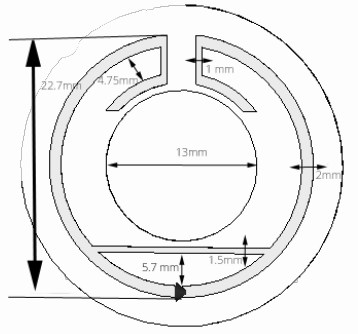
\includegraphics[width=5cm]{1STee}
\caption{Antenne à boucle}
\end{figure}
Comme le montre la figure 3.18 la taille a été énormément améliorée et les performances de cette antenne restent les mêmes. Cette structure nous a permit un bon contrôle de fréquence. Toute variation de longueur de 2mm nous donne un décalage de fréquence de 10MHz. La figure 3.19 est le S11 après chaque coupage de boucle intérieur de 2mm. Plus de détails sur la simulation seront présentés dans le chapitre suivant.\\\\\\\\

\begin{figure}[H]
\centering
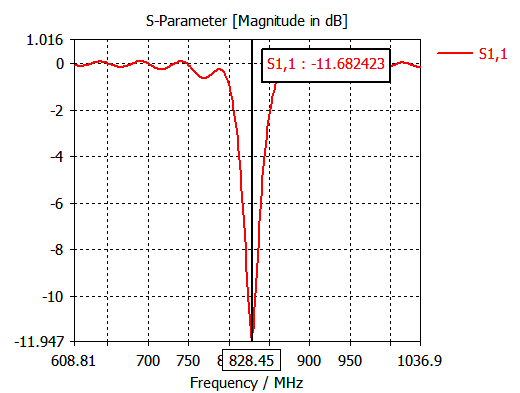
\includegraphics[width=6cm]{11}
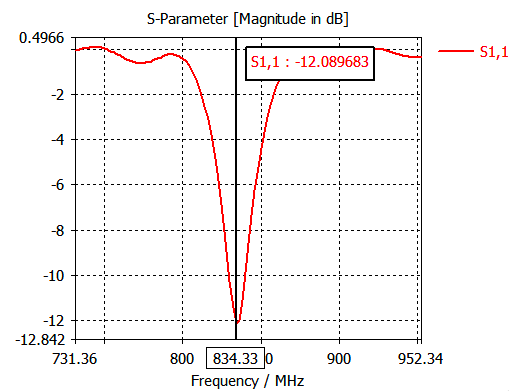
\includegraphics[width=6cm]{22}\\
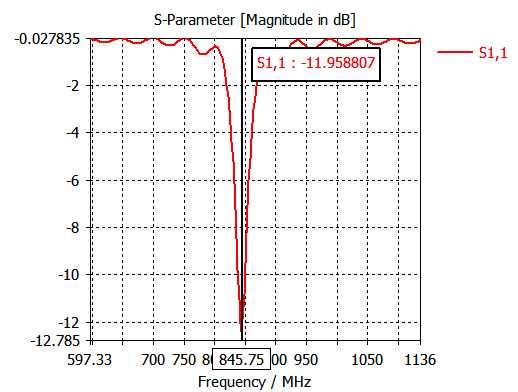
\includegraphics[width=6cm]{33}
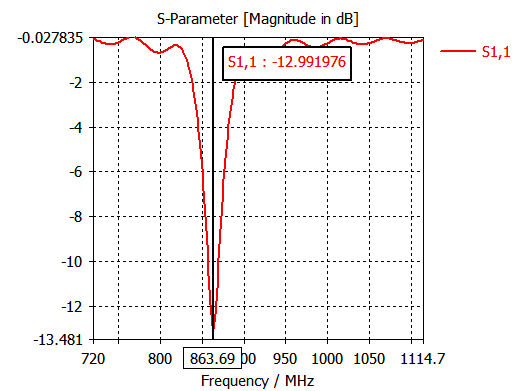
\includegraphics[width=6cm]{44}
\caption{S11 après coupage de 2mm }
\end{figure}

La troisième étape  consiste à réaliser l'antenne de la figure 3.17. 
Avant de concevoir un prototype du tag RFID destiné à la traçabilité des palettes, un modèle a été mis à notre disponibilité pour être analysé dans les laboratoires de MAScIR. Le but de cette analyse est de caractériser le produit et de déterminer les différents matériaux utilisés.\\

On commence par une analyse non destructive qui consiste à faire une analyse générale du boîtier puis une description générale du package vue de l’extérieur, puis avec les Rayons X comme illustré dans la figure 3.17. En suite on procède à l'analyse destructive qui consiste à décapsuler le package puis une décapsulation du système.\\

Dans la figure suivante. Cette structure a été inspirée de l'analyse avec x-ray d'une antenne achetée qui rayonne dans la fréquence 915MHz. L'expérience montre que sa distance de lecture est de 2m. Plus de détails sur la simulation seront présentés dans le chapitre suivant.\\

\begin{figure}[H]
\centering
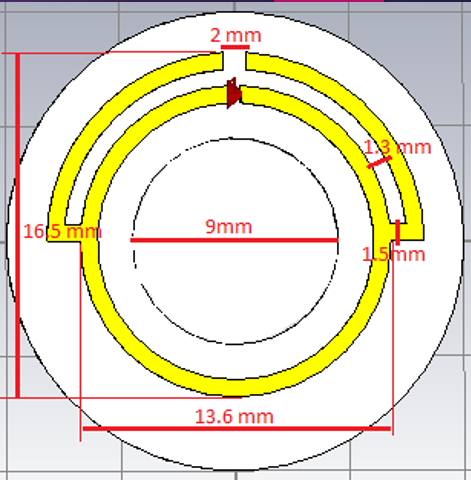
\includegraphics[width=4cm]{front11}
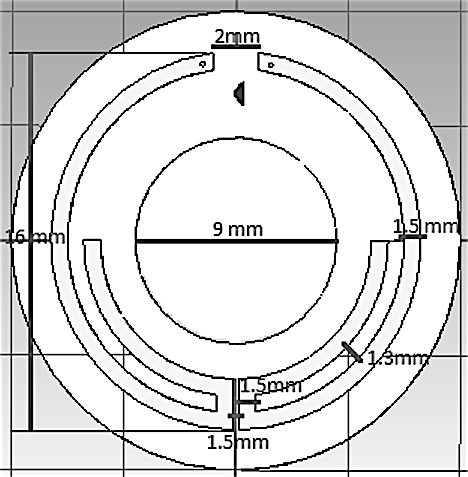
\includegraphics[width=4cm]{back22}
\caption{Antenne du X-ray}
\end{figure}
\subsection{Conclusion}
Dans ce chapitre on a présenter le protocole de communication qui assure la communication entre le lecteur et l'antenne. Ensuite on a parler de la solution Android pour le lecteur LF RFID finalement on a discuté les notions théorique qui régie les antennes à boucle circulaire qui représente une excellente solution pour les antennes de petite taille. Une étude sur les méthodes d'optimisation ont été détaillées dans cette section comme le \emph{Short stub} et le bouclage interne qui permettent de réduire la taille et garder le caractère omnidirectionnel, après cet étape on a élaboré un plan d'expérience qui consiste à examiner un tag acheté et puis l'analyser avec les \emph{X-RAYs} pour s'inspirer de sa structure. Le produit final de cet étude est un tag UHF marocain d'excellente performance.

\chapter{Réalisation et simulation des projets}
Ce chapitre comporte une présentation concernant 
les outils de réalisation et simulation 
la réalisation du projet
les étapes de test et de vérification 
le plan de mise en œuvre et le plan de maintenance.
\section{Outils	de	réalisation	et de	simulation}
\subsection{Visual Studio et .net C\#}
\subsubsection{Visual Studio}
Microsoft Visual Studio est un environnement de développement intégré (IDE) de Microsoft. Il est utilisé pour développer des programmes informatiques pour Microsoft Windows, ainsi que des sites Web, des applications Web et des services Web. Visual Studio utilise les plates-formes de développement de logiciels Microsoft tels que l'API Windows, Windows Forms, Windows Presentation Foundation, Windows Store et Microsoft Silverlight. Il peut produire à la fois le code natif et le code managé.

Visual Studio inclut un éditeur de code de support IntelliSense (le composant de complétion de code) ainsi que le code refactoring. Le débogueur intégré fonctionne à la fois comme un débogueur de niveau source et un débogueur de niveau de la machine. D'autres outils intégrés comprennent un concepteur de formulaires pour les applications bâtiment de l'interface graphique, web designer, concepteur de la classe, et concepteur de schéma de base de données. Il accepte les plug-ins qui améliorent la fonctionnalité à presque tous les niveaux, y compris l'ajout du support pour les systèmes de commande source (comme Subversion) et l'ajout de nouveaux jeux d'outils tels que les éditeurs et les concepteurs visuels pour les langues spécifiques au domaine ou toolsets pour d'autres aspects du cycle de vie du développement logiciel (comme le client Team Foundation Server: Team Explorer).

Visual Studio supporte différents langages de programmation et permet à l'éditeur de code et débogueur pour support  presque tout langage de programmation, C, C ++, VB.NET (Visual Basic .NET), C sharp (via Visual C \#), et F \# (à partir de Visual Studio 2010  ). Le support d'autres langages tels que Python, Ruby, Node.js, et autres est disponible via les services linguistiques installés séparément. Il prend également en charge XML / XSLT, HTML / XHTML, JavaScript et CSS. Java (et J \#) ont été pris en charge dans le passé.

\begin{figure}[H]
\centering
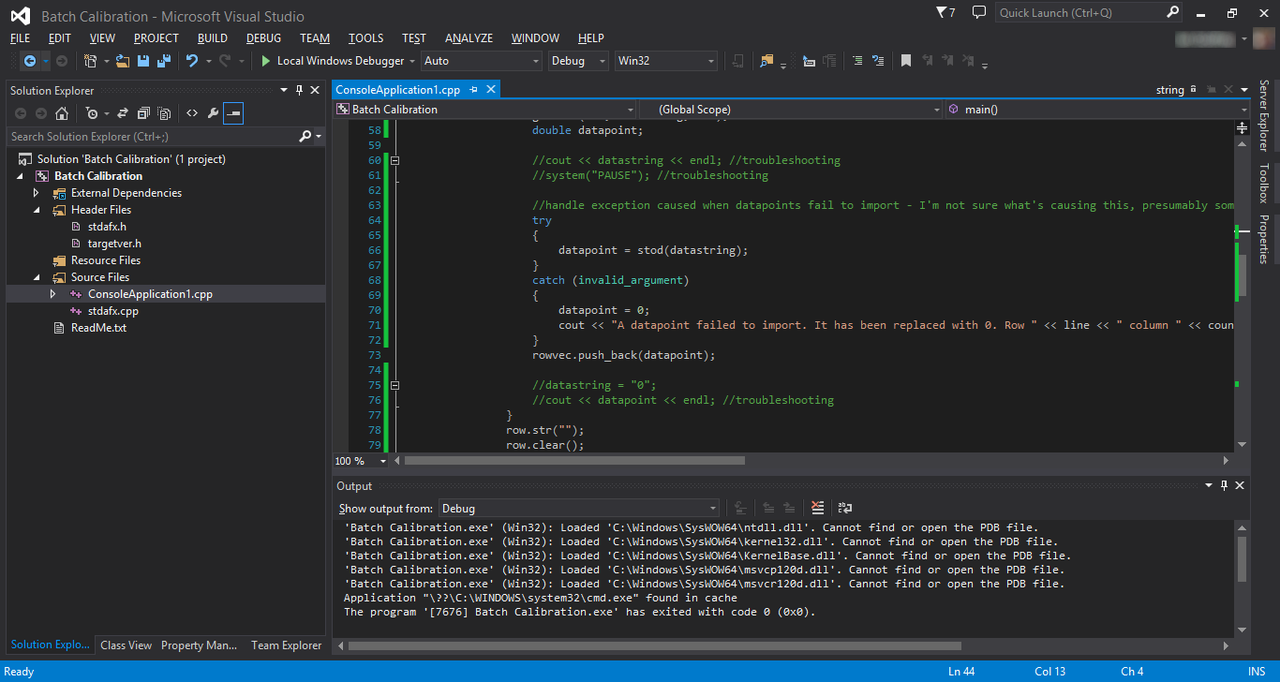
\includegraphics[width=\textwidth]{vs}
\caption{Interface Visual studio }
\end{figure}

\subsubsection{.net C \#}
C \# est un langage orienté objet élégant et sécurisé qui permet aux développeurs de créer une variété d'applications robustes qui fonctionnent sur le .NET Framework. Vous pouvez utiliser C \# pour créer des applications Windows client, les services Web XML, composants distribués, les applications client-serveur, les applications de base de données, et beaucoup, beaucoup plus. Visual C \# fournit un éditeur avancé de code, les concepteurs d'interface utilisateur pratique, débogueur intégré, et bien d'autres outils pour faciliter le développement d'applications basées sur le langage C \# et .NET Framework.\\

Les programmes C \# exécutés sur le .NET Framework, une partie intégrante de Windows qui inclut un système d'exécution virtuel appelé le Common Language Runtime (CLR) et un ensemble unifié de bibliothèques de classes. Le CLR est la mise en œuvre commerciale par Microsoft de l'infrastructure de langage commun (CLI), une norme internationale qui est la base pour la création des
environnements d'exécution et de développement dans lequel les langues et les bibliothèques travaillent ensemble de façon transparente.\\

Le code source écrit en C \# est compilé dans un langage intermédiaire (IL) qui est conforme à la spécification CLI. Le code et les ressources IL, tels que des bitmaps et des chaînes, sont stockés sur le disque dans un fichier exécutable appelé un ensemble, généralement avec une extension .exe ou .dll. Un assemblage contient un manifeste qui fournit des informations sur les types de l'assemblage, la version, la culture, et les exigences de sécurité.\\

Lorsque le programme C \# est exécuté, l'ensemble est chargé dans le CLR, ce qui pourrait prendre diverses mesures basées sur les informations contenues dans le manifeste. Ensuite, si les conditions de sécurité sont remplies, le CLR effectue juste à temps (JIT) pour convertir le code IL aux instructions machine natives. Le CLR fournit également d'autres services liés à la collecte automatique des déchets, la gestion des exceptions, et la gestion des ressources. Le code qui est exécuté par le CLR est parfois appelé « code managé," contrairement à "code non managé » qui est compilé en langage machine natif qui cible un système spécifique. Le schéma suivant illustre la compilation et l'exécution des relations de fichiers source C \# de code, les bibliothèques de classes .NET Framework, les assemblages et le CLR.
\begin{figure}[H]
\centering
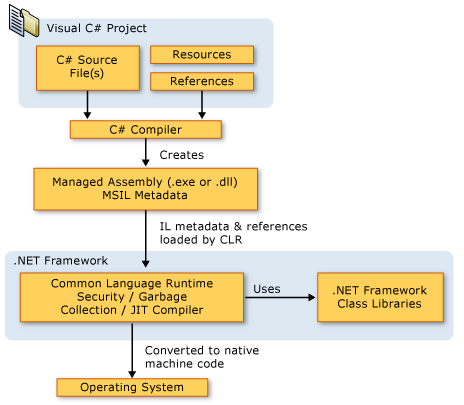
\includegraphics[width=9cm,height=9cm]{net}
\caption{Architecture du Framework .net}
\end{figure}
\subsection{Android Studio}
Android Studio est l'environnement de développement intégré officiel (IDE) pour le développement de la plate-forme Android. Il a été annoncé le 16 mai 2013 à la conférence Google I / O. Android Studio est disponible gratuitement sous la licence Apache 2.0. Android Studio a été au début de l'étape accès à l'aperçu à partir de la version 0.1 en mai 2013, puis il est entré en phase bêta à partir de la version 0.8 qui a été publié en Juin 2014. La première version stable a été publié en Décembre 2014, à partir de la version 1.0.\\

Basé sur le logiciel IntelliJ IDEA de JetBrains, Android Studio est conçu spécifiquement pour le développement Android. Il est disponible en téléchargement sur Windows, Mac OS X et Linux, et remplacé Outils Eclipse développement Android (HAA) comme IDE primaire de Google pour le développement d'applications Android native.\\


Les nouvelles fonctionnalités devraient être déployées avec chaque version d'Android Studio. Les fonctions suivantes sont fournies dans la version stable actuelle: 
\begin{itemize}
\item Gradle-based  renforcer et soutenue.
\item Refactoring Android-spécifique et des solutions rapides.
\item Outils de monitoring de performance, facilité d'utilisation et la compatibilité de version 
\item Assistants basés sur des modèles pour créer des dessins et des composants 
\item Un riche éditeur de mise en page qui permet aux utilisateurs de glisser-déposer les composants de l'interface
\item Soutien pour la construction des applications Android
\item Support intégré pour Google Cloud Platform, intégration permettant à Google Cloud Messaging et App Engine.
\end{itemize}
\begin{figure}[H]
\centering
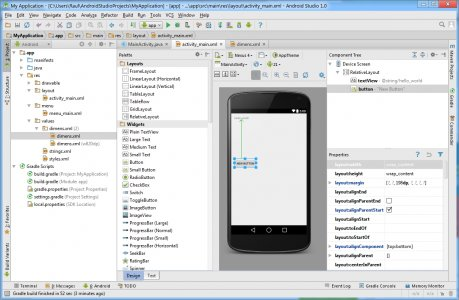
\includegraphics[width=\textwidth]{as}
\caption{Interface d'Android Studio}
\end{figure}

\subsection{CST studio}
CST MICROWAVE STUDIO (CST MWS) est un outil spécialisé pour la simulation 3D EM de composants à haute fréquence. Une performance inégale de CST MWS  ce qui fait de lui le premier choix dans la technologie de radio fréquence.\\

CST MWS permet l'analyse rapide et précise de haute fréquence (HF) des dispositifs comme des antennes, des filtres, coupleurs, plans et les structures multicouches.  CST MWS vous donne rapidement un aperçu du comportement EM de nos conceptions à haute fréquence.\\

CST support la technologie complète pour la 3D EM. Le solveur \emph{Time Domain} est largement applicable et le solveur de \emph{domaine de fréquence}, CST MWS offre d'autres modules de solveurs pour des applications spécifiques. \\

CST MICROWAVE STUDIO est vu par un nombre croissant d'ingénieurs comme un outil du développement standard de l'industrie.
\begin{figure}[H]
\centering
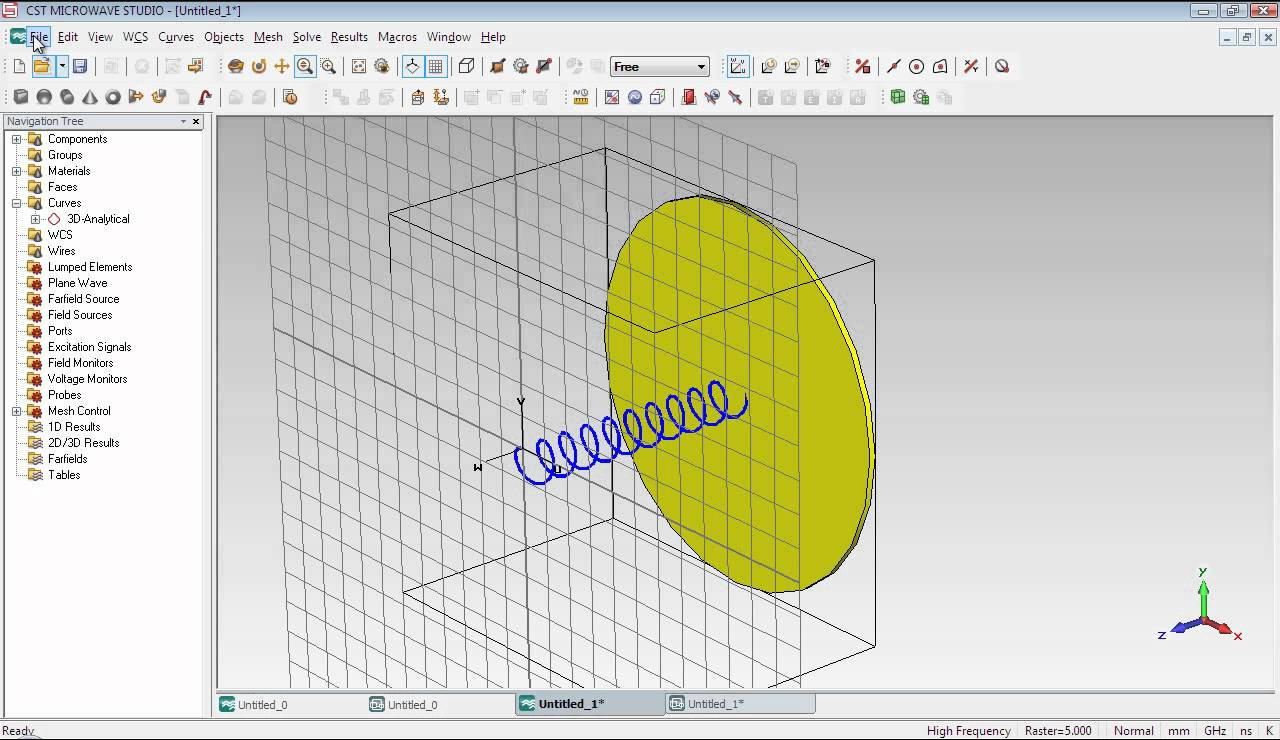
\includegraphics[width=\textwidth]{cst}
\caption{Interface CST studio}
\end{figure}
\section{Test	 et vérification	}
\subsection{RFID Desktop}
L'application desktop  est un logiciel pour la gestion des entrées et sorties des palettes du stock. Elle exécute au sein d'elle le protocole qu'on appel l'interface RFID qui à son tour communique avec le lecteur et le commande afin de bien gérer sont interface air. Les détails de cette interface sont décrites dans le chapitre précédant. 
\begin{figure}[H]
\centering
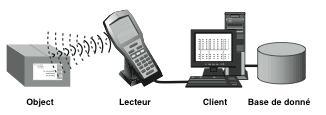
\includegraphics[width=9cm]{systemx}
\caption{Rappel du système RFID}
\end{figure}
Dans la figure prétendante je ai rappelé l'architecture globale d'un système RFID. Notre interface ce positionne entre le lecteur et la base de données. Cette interface permet l'acquisition des données du lecteur et les présenter dans une forme logique au utilisateur.
\subsubsection{Interface utilisateur et option de stockage}
L'interface utilisateur permet une visualisation claire et organisée des données elle permet aussi la gestion du serveur de base de données et les méthodes de sécurité de cette communication aussi les ajouts des dépendances comme l'état de tag (in ou out), elle permet aussi d'ajouter la date quand le tag a été lu. La figure suivante est l'interface qui donne la main à l'utilisateur de contrôler sa base de données.\\

\begin{figure}[H]
\centering
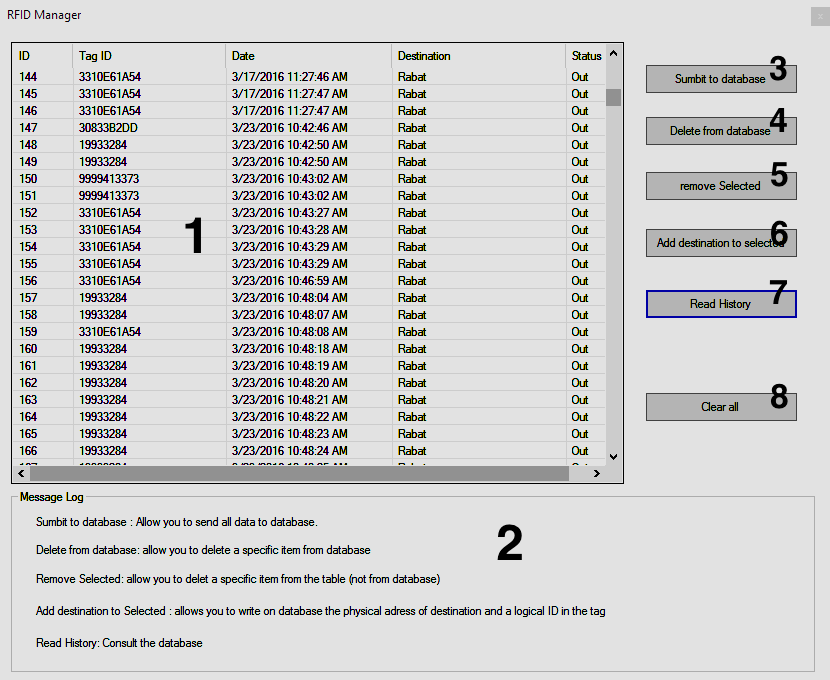
\includegraphics[width=\textwidth]{software}
\caption{L'interface utilisateur}
\end{figure}
La liste \(^{1}\), représente un espace où l'utilisateur peut visualiser les résultats de ses requêtes. Elle est repartie en six champs. l'ID est l'identifiant du palette au sein du système de base de données. Les raisons derrière le choix de créer un nouveau ID et ne pas utiliser celui du tag sont les suivantes:
\begin{itemize}
\item Il est plus rapide. À JOIN sur un nombre entier est beaucoup plus rapide que JOIN sur un champ de chaîne ou une combinaison de champs. Il est plus efficace de comparer des nombres entiers que les chaînes de caractères.

\item Il est plus simple. Il est beaucoup plus facile de cartographier des relations fondées sur un champ numérique unique que sur une combinaison d'autres domaines de différents types de données.

\item Ce sont des données indépendantes.

\item  Il est plus efficace si on cherche à effectuer un trie.\\
\end{itemize}


Le champ \(^{2}\) est un log qui permet de transmettre des informations très utiles pour l'utilisateur. Comme le rôle de chaque bouton et comment interagir avec le logiciel. Le bouton \(^{3}\) donne la possibilité à l'utilisateur de soumettre tout le contenu du champ liste à la base de données d'une manière simple et sécurisée sans perte d'information. Le bouton \(^{4}\) permet à l'utilisateur de mieux gérer sa base de données en donnant la possibilité de supprimer un champ bien spécifique de la liste et de la base de données. Cette possibilité va faciliter la maintenance des données dans notre base et éviter les répétition en cas d'erreur de lecture. Le bouton \(^{5}\) permet à l'utilisateur de supprimer les données de la list sans les supprimer de la base de données. Le bouton \(^{6}\) est une fonctionnalité très intéressante elle permet à l'utilisateur d'affecter une destination à un ou plusieurs champs de la liste. Cette fonctionnalité permet une traçabilité claire des palettes. Le bouton\(^{7}\) est la fonctionnalité d'historique elle permet de lire toutes les données de la base de données et les afficher dans la liste avec toutes les attribues relative à ces données.
le bouton \(^{8}\) permet la suppression des données affichées dans la liste sans les supprimer de la base de données.

\subsection{Application Android - SmartFlah}
Dans cette section je vais parler du deuxième projet qui consiste à développer une application Android pour le tag LF, ses fonctionnalités qui vont faciliter la vie d'un consommateur comme un éleveur ou producteur de viande rouge. Les figures suivantes toutes les \emph{layouts} de note application. Une explication détaillée des fonctionnalités sera présentée après. La figure suivante présente le lecteur LF RFID et le tag.

\begin{figure}[H]
\centering
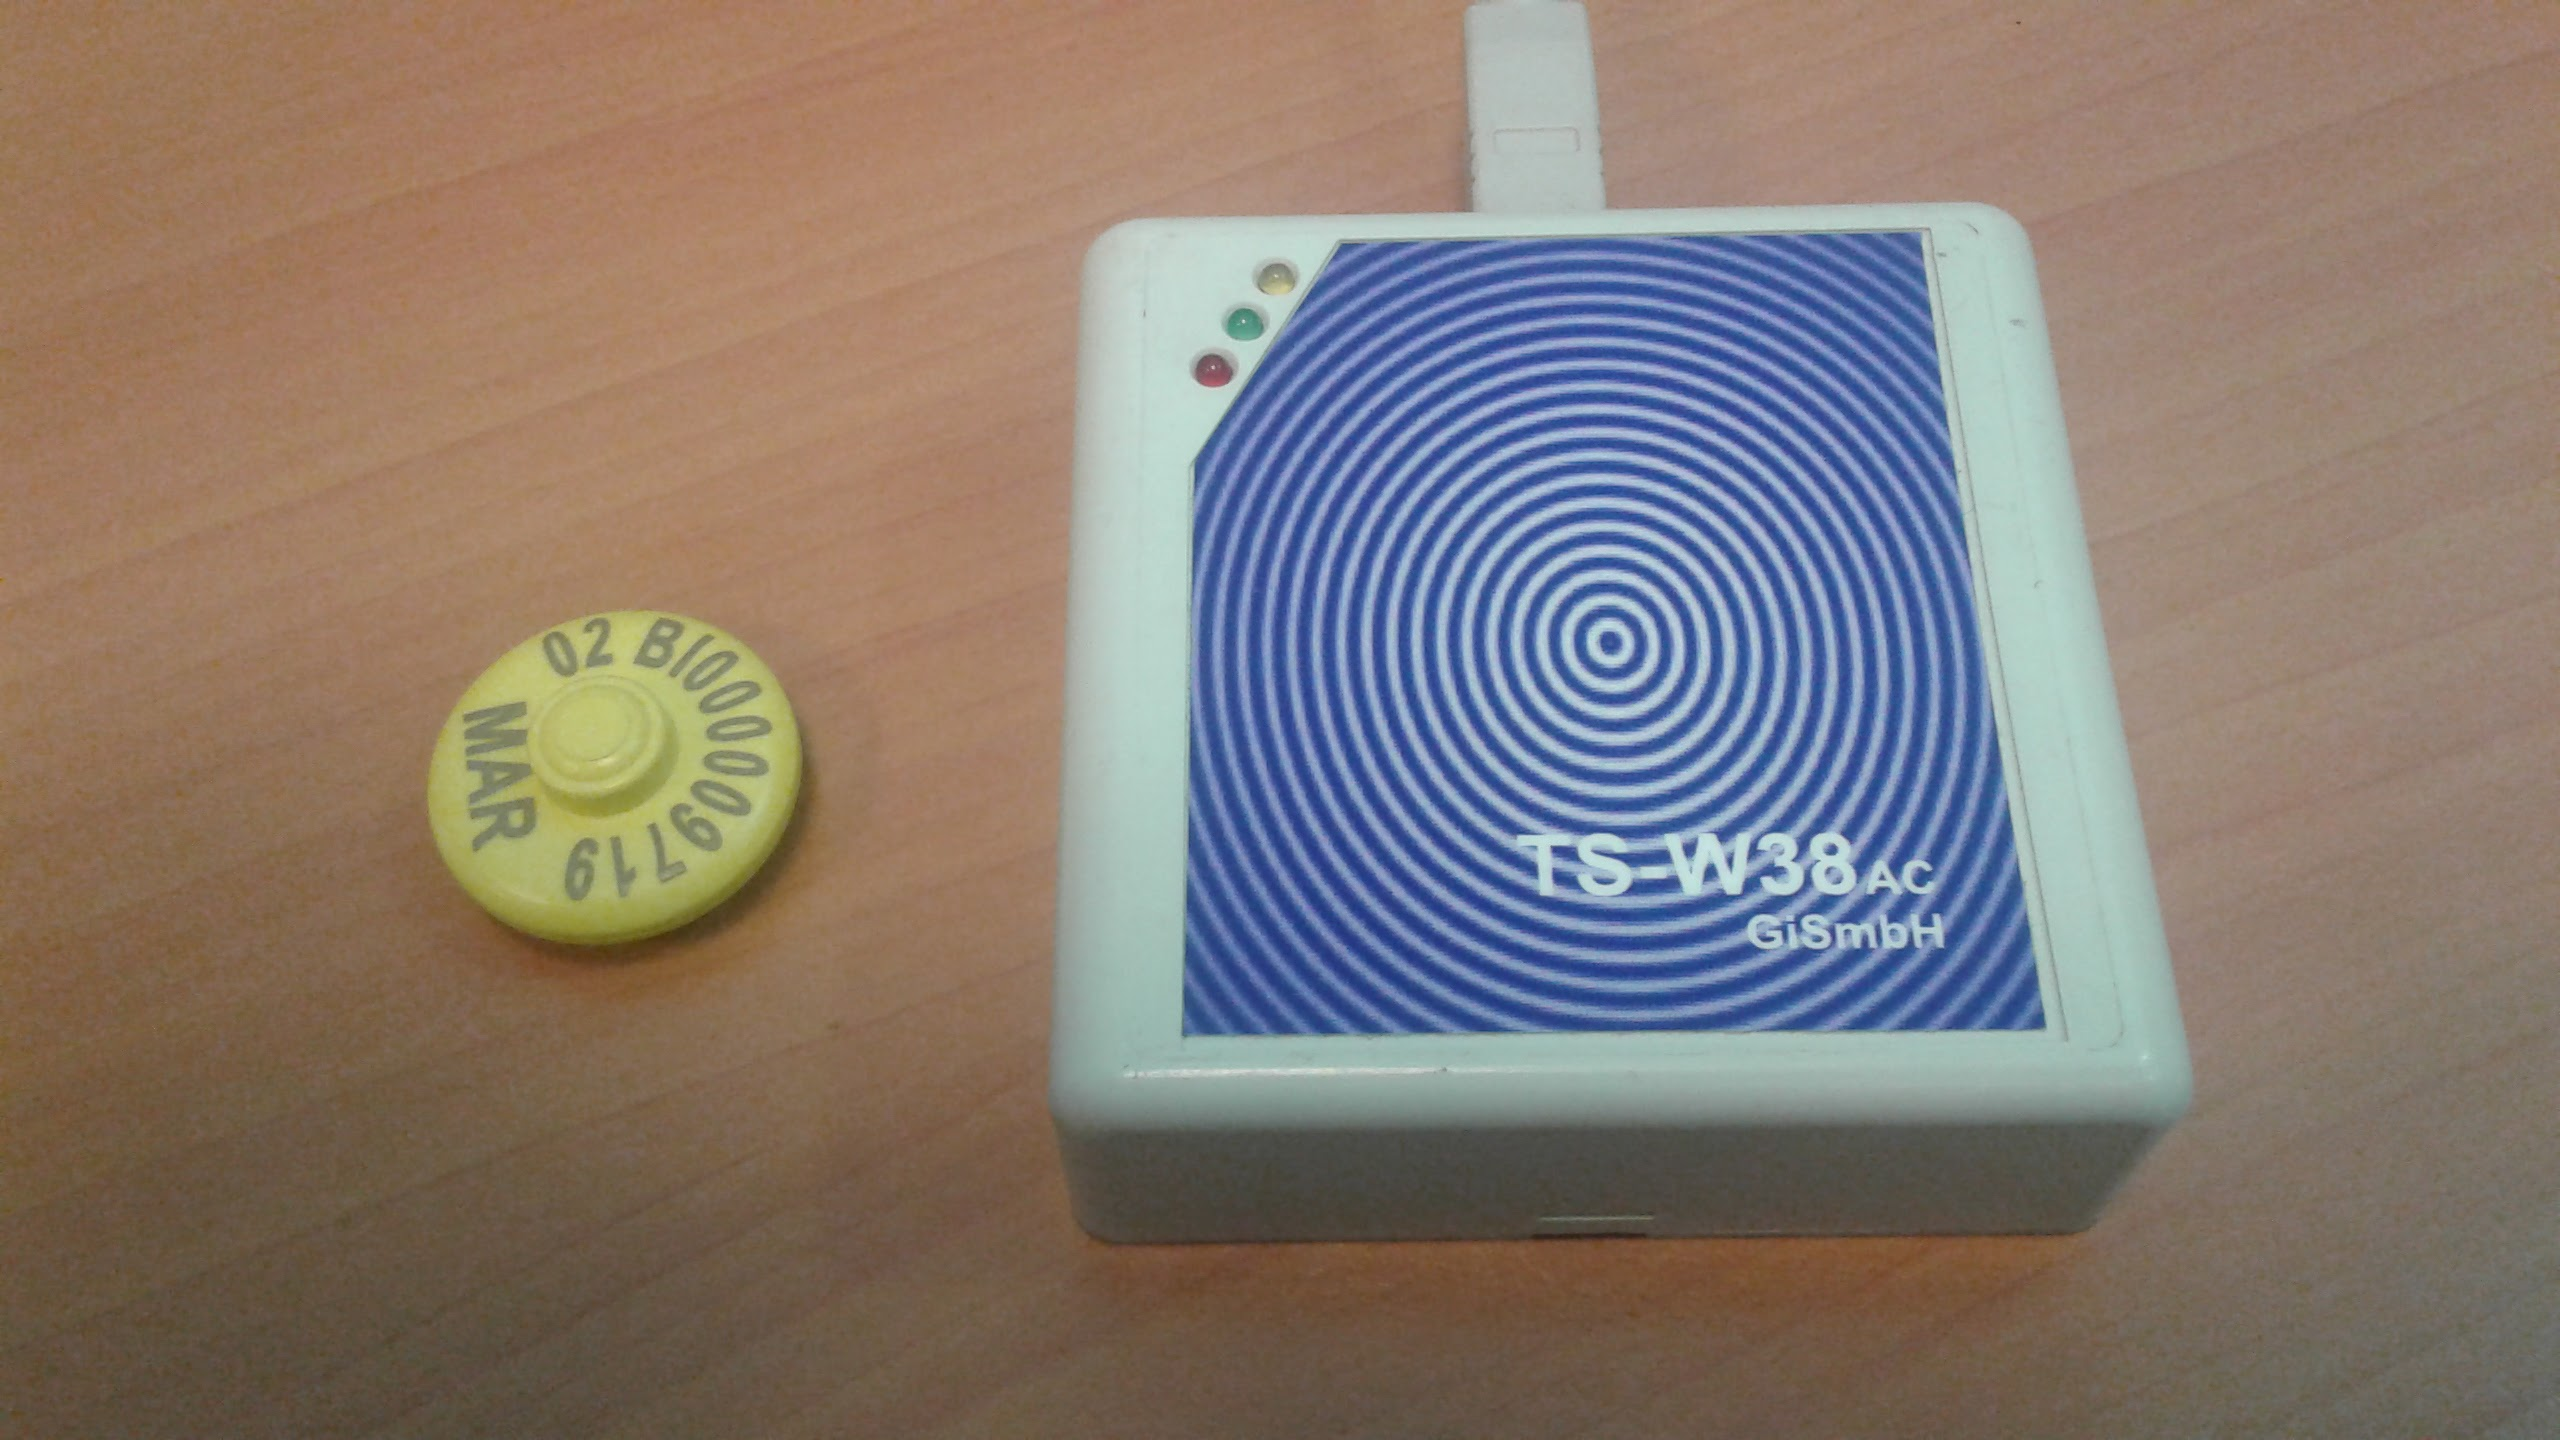
\includegraphics[width=\textwidth]{lfreader}
\caption{LF RFID system}
\end{figure}

\subsubsection{Interface Android et Fonctionnalité}
La figure suivante est la première \emph{layout} qui s'affiche après le lancement de l'application. Dans cette \emph{layout} on affiche le ID lu par le lecteur LF avec la possibilité de le valider \(^{1}\) . L'interface propose trois possibilités pour l'utilisateur: l'envoi \(^{2}\) du rapport des IDs lus au serveur distant, elle donne la possibilité aussi de naviguer\(^{3}\) d'autre option avec un simple glisse à droite.
\begin{figure}[H]
\centering
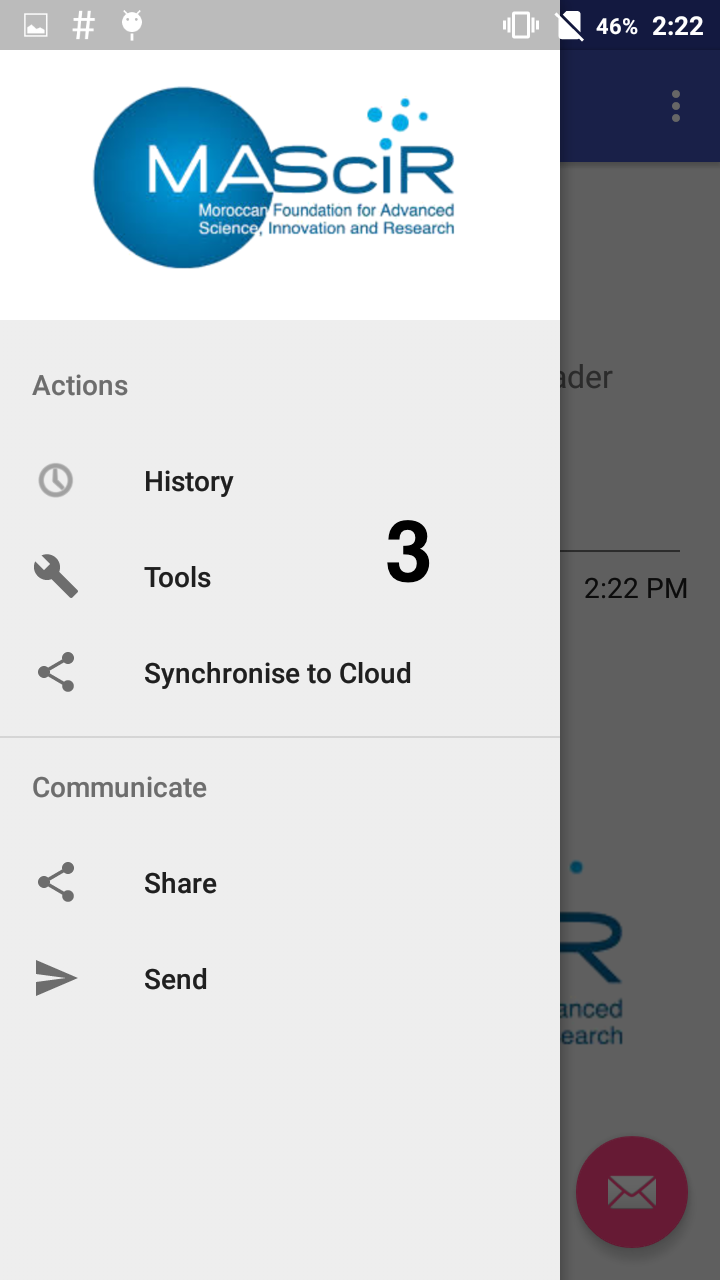
\includegraphics[width=4.4cm,height=8cm]{rightmenu}
\includegraphics[width=4.4cm,height=8cm]{1}
\caption{Première layout}
\end{figure}

Après la validation de l'ID, deux scénarios se manifestent. Sois l'ID existe dans la base de données donc on affiche\(^{5}\) toutes les données relatives à ce tag ou bien c'est un nouveau ID qui nécessite une saisie\(^{4}\) des données relative à ce dernier. L'application ajoute directement des données relative à la position actuelle en utilisant le système GPS \footnote{Global Positioning System} les deux figures suivantes représentent les \emph{layouts} qui prennent en charge ces fonctionnalités.

\begin{figure}[H]
\centering
\includegraphics[width=4.4cm,height=8cm]{showdialog}
\includegraphics[width=4.4cm,height=8cm]{form}
\caption{Layout de forme et affichage}
\end{figure}

L'application permet aussi de sauvegarder les données dans une base de données interne dans le téléphone et aussi dans des serveurs distants. L'application offre trois services de partage et sauvegarde des données (Gmail,Drive).L'application permet aussi le partage des données avec un autre périphérique en utilisant (Bleutouth,Beams). Dans la version récente on peut partager en utilisant (imo et whatapp).
 
 \begin{figure}[H]
\centering
\includegraphics[width=4.4cm,height=8cm]{sharemenu}
\includegraphics[width=4.4cm,height=8cm]{gmail}
\includegraphics[width=4.4cm,height=8cm]{drive}
\caption{Layout de Partage}
\end{figure}

\subsection{Antenne UHF}

Pour décrire la performance d'une antenne , les définitions des différents paramètres sont nécessaires . Certains paramètres sont interdépendants et tous entre eux doivent être indiquées pour une description complète de la performance de l'antenne. La définition des paramètres sera donnée dans la section suivante. Beaucoup de paramètres sont des standards IEEE  ( IEEE Std 145-1983 ). Ensuite je vais présenter les différentes résultats et simulations sur les antennes RFID UHF. La puce utilisée est la H3 de Alien. Le logiciel simulation est CST studio 2014 qui permet de calculer un grand nombre des paramètres d'antenne.\\
\subsubsection{Les paramètres de l'antenne}
\begin{itemize}
\item \emph{RADIATION PATTERN} est une fonction mathématique ou une représentation graphique des propriétés de rayonnement de l'antenne en fonction des coordonnées spatiales. Dans la plupart des cas, le diagramme de rayonnement est déterminé dans la région de champ \emph{Far-Field} est représenté comme une fonction des coordonnées de direction . Les propriétés du rayonnement comprennent la densité du flux de puissance, l'intensité du rayonnement, l'intensité du champ et directivité de phase ou de polarisation.\\\\\\\\
\begin{figure}[H]
\centering
\includegraphics[width=5cm,height=5cm]{radpa}
\caption{Radiation pattern}
\end{figure}
\item \emph{la directivité} retour d'une antenne est définie comme: le rapport de l'intensité du rayonnement dans une direction donnée de l'antenne à l'intensité de rayonnement moyen de toutes les directions. L'intensité du rayonnement moyen est égale à la puissance totale rayonnée par l'antenne divisée par 4\(\pi\) . En forme mathématique elle peut être écrite comme:

\begin{equation}
D = \dfrac{U}{U_{0}} = \dfrac{4 \pi U}{P_{rad}}
\end{equation}

Si la direction n'est pas spécifiée, elle implique la direction de l'intensité maximale de rayonnement( Directivité maximum) exprimé comme:

\begin{equation}
D_{max} = D_{0} = \dfrac{U}{U_{0}} = \dfrac{4 \pi U_{max}}{P_{rad}}
\end{equation}
D = directivité (sans dimension)\\
\(D_{0}\) = directivité maximale (sans dimension)\\
U = intensité du rayonnement ( W / unité d'angle solide )\\
\(U_{max}\) = intensité maximale de rayonnement ( W / unité d'angle solide )\\
\(U_{0}\) = intensité du rayonnement de la source isotrope ( W / unité d'angle solide ) Prad = puissance totale rayonnée ( W )\\

\item \emph{EFFICACITÉ} elle peut être définit comme suite: \emph{comment bien l' antenne rayonne la puissance qui lui a été donnée.} L'efficacité totale de l'antenne est utilisée pour prendre en compte les pertes au niveau des bornes d'entrée et à l'intérieur de la structure de l'antenne. Ces pertes peuvent être dues à la réflexion en raison de mal adaptation entre la ligne de transmission et la source de l'antenne, la conduction et diélectrique

\begin{figure}[H]
\centering
\includegraphics[width=4cm,height=3cm]{wellwellwell}
\caption{réflexion,conduction,perte de diélectrique}
\end{figure}
D'une manière générale, le rendement global peut être écrit comme:

\begin{equation}
e_{0}=e_{r}e_{c}e_{d}
\end{equation}

\(e_{0}\) = l'efficacité totale ( dimension)\\
\(e_{r}\) = réflexion \emph{ mismatch} \\
\(e_{c}\) = l'efficacité de conduction ( sans dimension)\\
\(e_{d}\) = efficacité diélectrique ( sans dimension)\\

\item \emph{VSWR} 
Pour une radio ( émetteur ou récepteur ) pour délivrer une puissance à une antenne, l'impédance de la ligne de transmission radio doit être bien adaptée à l'impédance de l'antenne. Le paramètre ROS ou VSWR est une mesure qui décrit numériquement la façon dont l'antenne est adaptée d'impédance à la ligne de la radio ou de la transmission quand elle est connectée.
\begin{equation}
VSWR = \dfrac{1+ |\Gamma|}{1-|\Gamma|}
\end{equation}

\item \emph{S paramètres}
décrivent la relation d'entrée-sortie entre les ports (ou terminaux) dans un système électrique . Par exemple, si nous avons 2 ports ( intelligemment appelé Port 1 et Port 2), puis S12 représente la puissance transférée de Port 2 à Port 1. S21 représente la puissance transférée de Port 1 à Port 2. En général, SNM représente la puissance transférée de Port M à Port N dans un réseau multi-port.
\end{itemize}

\subsubsection{Antenne à inductance}


L'étiquette UHF considérée est constituée d’une antenne à dipôle électrique avec une piste courbe d’inductance à travers le dipôle à des fins d'adaptation d'impédance. La structure et les dimensions de cette balise sont représentées sur la figure 5.13. Cette balise est faite en utilisant une carte FR4 avec une épaisseur de substrat h = 1,6 mm et de permittivité diélectrique \(\epsilon_{r}\) = 4,4. Cette conception de l’étiquette est de simple face. L'impédance simulée est de 20 + j152 \(\Omega\) est tout à fait adaptée.\\
 
 \begin{figure}[H]
\centering
\includegraphics[width=6cm]{dofi}\\
\caption{Antenne à inductance}
\end{figure} 

Les figures suivantes représente les quatre paramètres qui caractérisent une antenne. La figure 4.14 illustre
la variation du paramètre de réflexion en fonction de la fréquence, à 910 MHz l'antenne pressente une valeur importante de -20 db de S11, ce qui présente 99\% de la puissance est rayonné de la source vers l'air. Le diagramme de rayonnement  nous donne une directivité supérieur a 1.5 dbi, pour le cas de notre application c'est idéal. A la pratique pour valeur de VSWR inférieur à 3 on considère que c'est un résultat acceptable, dans la figure 4.16  on relevé une valeur de VSWR inférieur à 2 pour la fréquence de résonance de l'antenne. La dernière figure représente l'efficacité du matériaux dans notre cas le cuivre. une valeur de -2 dB est largement acceptable.
\begin{figure}[H]
\centering
\includegraphics[width=10cm,height=4cm]{clas11}
\caption{S-paramètres de l'antenne à inductance}
\end{figure} 




\begin{figure}[H]
\centering
\includegraphics[width=10cm,height=5cm]{clapolfarfield}
\caption{Diagramme de rayonnement de l'antenne à inductance}
\end{figure} 


\begin{figure}[H]
\centering
\includegraphics[width=10cm,height=4cm]{clavswr}
\caption{VSWR de l'antenne à inductance}
\end{figure} 

\begin{figure}[H]
\centering
\includegraphics[width=10cm,height=4cm]{claefficency}
\caption{Efficacité de l'antenne à inductance}
\end{figure} 


%talke about seuille values and compared them to what we got
% bandwith power related to s11, (feathers or capabilities)

\subsubsection{L'antenne à boucle circulaire}
La structure suivante représente la forme améliorée de l'antenne précédente, cette structure nous a permit de réduire la taille et mettre la main sur un contrôle totale de fréquence. L'impédance de l'antenne simulée est  de 27 + j180\(\Omega\)
.
\begin{figure}[H]
\centering
\includegraphics[width=6cm]{1STee}
\caption{Antenne à boucle circulaire}
\end{figure}

Les figures suivantes représente les quatre paramètres qui caractérisent une antenne. La figure 4.19 illustre
la variation du paramètre de réflection en fonction de la fréquence, à 867 MHz l'antenne présente une valeur importante de S11 de -12 db, ce qui donne que 90\% de la puissance est rayonné de la source vers l'air. Le diagramme de rayonnement  nous donne une directivité supérieur à 1.47 dbi, pour le cas de notre application c'est idéal. Une valeur du VSWR inférieur à 3 est  considérer acceptable, dans la figure 4.21  on relevé une valeur inférieur 1.55 dans la fréquence de résonance  de l'antenne. La dernier figure représente l'efficacité du matériaux dans notre cas le cuivre. une valeur de -1.5 dB est largement acceptable.

\begin{figure}[H]
\centering
\includegraphics[width=10cm,height=4cm]{claaaass11}
\caption{S-paramètres de l'antenne à  boucle circulaire}
\end{figure} 

\begin{figure}[H]
\centering
\includegraphics[width=10cm,height=5cm]{claPattern}
\caption{Diagramme de rayonnement de l'antenne à  boucle circulaire}
\end{figure} 

\begin{figure}[H]
\centering
\includegraphics[width=10cm,height=4cm]{claaavswr}
\caption{VSWR de l'antenne à  boucle circulaire}
\end{figure} 

\begin{figure}[H]
\centering
\includegraphics[width=10cm,height=4cm]{clawefficency}
\caption{Efficacité de l'antenne à  boucle circulaire}
\end{figure} 

%talke about seuille values and compared them to what we got
% bandwith power related to s11, (feathers or capabilities)

La figure suivante présente les résultats du \emph{Reverse engineering}. L’étiquette est constituer de deux couches de cuivre, la puce est fixée sur l'antenne  avec \emph{wire bonding}. \\

\begin{figure}[H]
\centering
\includegraphics[width=4cm]{front11}
\includegraphics[width=4cm]{back22}
\caption{Antenne du X-Ray}
\end{figure}

Les figures suivante représente les quatre importante paramètres à prendre en considération pour le jugement d'une antenne. S paramètres décrivent la relation d'entrée-sortie entre les ports (ou terminaux). S11 de notre système est d'environ -21 dB pour la fréquence de 915 MHz La bande passante est de 5MHz. Le VSWR ou ROS (Voltage Ratio ondes stationnaires) décrit la puissance réfléchie par l'antenne. Quand VSWR est de 1,0, aucune puissance est réfléchie, ce qui est idéal. Pour l'antenne proposé ROS = 1.5. Le diagramme de rayonnement se réfère à la direction (angulaire) la dépendance de l'intensité des ondes radio provenant de l'antenne ou d'une autre source. La figure ci-dessous montre une directivité de 1.95dbi.

\begin{figure}[H]
\centering
\includegraphics[width=10cm,height=4cm]{uses11}
\caption{S-paramètres de l'antenne X-Ray}
\end{figure} 

\begin{figure}[H]
\centering
\includegraphics[width=10cm,height=5cm]{usefar}
\caption{Diagramme de rayonnement de l'antenne X-Ray}
\end{figure} 

\begin{figure}[H]
\centering
\includegraphics[width=10cm,height=4cm]{useeff}
\caption{Efficacité de l'antenne X-Ray}
\end{figure} 
%talke about seuille values and compared them to what we got
% bandwith power related to s11, (feathers or capabilities)
\subsection{Conclusion}
Dans ce chapitre j'ai présenté tous les outils de simulation que j'ai utilisé que ça soit pour la partie programmation ou simulation des antenne, ainsi que la description de toutes les fonctionnalités des interfaces graphique et les paramétrés de simulation de toutes les antennes.

\chapter*{Conclusion}
\addcontentsline{toc}{section}{Conclusion}
Lors de mon stage qui a duré quatre mois à MAScIR, j'ai eu l'occasion de travailler sur la technologie RFID. En commençant par l'étude et le choix des tags et lecteurs adaptés pour notre application.\\

La première étape était de développer un middle-ware et un protocole de communication qui assurent à la fois le contrôle du périphérique de la machine en assurant une claire visibilité du stock. Le langage de programmation choisi était C\# car c'est un langage complet et se base sur la framework .net.\\

La deuxième étape était de développer une application Android pour les lecteurs LF. L'application permet la lecture et le stockage des données lues. Elle donne la possibilité de partager les informations enregistrées dans des serveurs distants comme elle permet le partage avec d'autres périphériques grâce à son support de l'interface bluetooth.\\

L'étape finale de mon stage était de concevoir un transpondeur pour les applications RFID UHF. En se basant sur deux méthodes, le reverse engineering pour avoir une idée sur les solutions qui existent déjà  la deuxième était de chercher des articles et essayer de les améliorer et les adapter à notre besoin.\\

Parmi les difficultés rencontrées, était l'insuffisance du temps restant pour passer au \emph{process} et puis l'étape finale de la réalisation. La miniaturisation pose toujours un problème industriel, on a eu du mal au début à produire des tags miniaturisés, mais finalement on a put miniaturisé notre antenne de 30\%.\\

\begin{thebibliography}{9}

\bibitem{antennatheory} 
C. A. Balanis, "Antenna Theory: Analysis and
Design",2ndEdition,1997,JohnWiley and Sons.
 



\bibitem{j}  J. Landt, “The history of RFID,” Potentials, IEEE, vol. 24, no. 4, pp. 8–11, 2005.

\bibitem{stub} Small Circular Loop Antenna for RFID Tag
Hong-Kyun Ryu and Jong-Myung Woo
Department of Radio Science and Engineering, College of Engineering, Chungnam National University, Daejeon, Korea

\bibitem{G} G. S. Pope, M. Y. Loukine, D. M. Hall, and P. H. Cole, “Innovative systems de- sign for 13.56 MHz RFID,” in Wireless and Portable Design Conference, Burling- ton, Massachusetts, 1997, pp. 240–245.

\bibitem{texas}  Texas Instruments, “Tag-it HF-I standard transponder IC - reference guide,” 15 Jan. 2007. 

\bibitem{alien}  “HF antenna design notes,” Technical Application Report, 2003.
[7] Alien Technologies, “915MHz EPC Class 1 RFID tags,” 15 Jan. 2007. [Online]. Available: http://www.alientechnology.com/products/documents/
alien 915mhz 128 bit.%pdf

\bibitem{fromat}  EPCglobal Tag Data Standards Version 1.3 Ratified Specification
March 8, 2006

\bibitem{air} EPC™ Radio-Frequency Identity Protocols Generation-2 UHF RFID
Specification for RFID Air Interface Protocol for Communications at 860 MHz – 960 MHz 
Version 2.0.0 Ratified

\bibitem{merize}  La méthode Merise : H. Tardieu, A. Rochfeld, R. Coletti aux Ed. d’organisation
AMC*Designor : Mise en œuvre de merise – Gilles GUEJ aux Editions Eyrolles
www.commentcamarche.net: La méthode Merise. 

\bibitem{iso} Information technology — Radio frequency identification for item management\\
Part 3: Parameters for air interface communications at 13,56 MHz
Technologies de l'information — Identification par radiofréquence (RFID) pour la gestion d'objets \\
Partie 3: Paramètres de communications d'une interface d'air à
13,56 MHz 
\bibitem{iso2}
Information technology — Radiofrequency identification for item management \\
Part 2:
Parameters for air interface
communications below 135 kHz 
\bibitem{iso6}
Information technology — Radio
frequency identification for item
management\\
Part 6:
Parameters for air interface
communications at 860 MHz to 960 MHz
General 

\bibitem{iso4}
Information technology — Radio
frequency identification for item
management\\
Part 4:
Parameters for air interface
communications at 2,45 GHz 

\bibitem{802.11b}
Overview of IEEE 802.11b Wireless LAN\\
S-72.4210 Postgraduate course in Radio Communications
10.1.2006\\
Tommi Koivisto
tommi.koivisto@tkk.f

\bibitem{802.15.4}
Zigbee / IEEE 802.15.4
Standard
Presenter: Dusan Stevanovic
June 20, 2007
\end{thebibliography}
\let\cleardoublepage\clearpage

\appendix
\printnomenclature
\chapter{Poster de SIAM}
\includepdf[pages=1]{post.pdf}

\chapter{Article IEEE}
\includepdf[pages=1]{bare_conf_compsoc.pdf}
\includepdf[pages=2]{bare_conf_compsoc.pdf}

\end{document}
